\chapter{Appendix}\label{appendix}

@@CL@@This appendix carries the material the body points at but has no room for, and a second group of results that did not reach Chapter 4 at all. Sections A to F support claims made in the text: the failure-mode register, the pipeline detail behind abstention and attribution, the experiment log, the questions ruled out in advance, the prior-work scoring, and the baselines. Sections G to J are new here: the full question bank, the catalogue recompute in full, the development-set results, and the figures the body does not use. Tables and figures are numbered by section, so Table C.1 is the first table of Appendix C.@@/CL@@

\section{A. Full Failure-Mode Register (FM-01 to FM-34)}\label{a.-full-failure-mode-register-fm-01-to-fm-34}

@@CL@@The register lists every way the project has identified for a wrong answer to reach the committed state. It was built by walking the pipeline stage by stage and asking what could pass each gate, not by collecting observed errors, so a mode can appear here without having fired in any run. Class is the useful column: \textquotesingle Caught\textquotesingle{} modes are stopped by a deterministic gate before commit, \textquotesingle LLM-only\textquotesingle{} modes are left as a prompt-tunable risk, and the twenty-two \textquotesingle Structural\textquotesingle{} modes cannot be closed by prompting alone. Those twenty-two are the count §5.4 cites and the attack list for further work.@@/CL@@

Severity is the product of likelihood and how silently a mode commits. `Caught' modes are stopped by a deterministic gate before commit; `LLM-only' modes are accepted as a prompt-tunable risk; `Structural' modes cannot be fixed by prompting alone @@CC@@and form the attack list for future work@@/CC@@.

{\def\LTcaptype{none} % do not increment counter
\begin{longtable}[]{@{}
  >{\raggedright\arraybackslash}p{(\linewidth - 10\tabcolsep) * \real{0.0685}}
  >{\raggedright\arraybackslash}p{(\linewidth - 10\tabcolsep) * \real{0.4302}}
  >{\raggedright\arraybackslash}p{(\linewidth - 10\tabcolsep) * \real{0.1372}}
  >{\raggedright\arraybackslash}p{(\linewidth - 10\tabcolsep) * \real{0.1274}}
  >{\raggedright\arraybackslash}p{(\linewidth - 10\tabcolsep) * \real{0.0899}}
  >{\raggedright\arraybackslash}p{(\linewidth - 10\tabcolsep) * \real{0.1469}}@{}}
\toprule\noalign{}
\begin{minipage}[b]{\linewidth}\raggedright
\textbf{ID}
\end{minipage} & \begin{minipage}[b]{\linewidth}\raggedright
\textbf{Failure mode}
\end{minipage} & \begin{minipage}[b]{\linewidth}\raggedright
\textbf{Stage}
\end{minipage} & \begin{minipage}[b]{\linewidth}\raggedright
\textbf{Class}
\end{minipage} & \begin{minipage}[b]{\linewidth}\raggedright
\textbf{Severity}
\end{minipage} & \begin{minipage}[b]{\linewidth}\raggedright
\textbf{Status}
\end{minipage} \\
\midrule\noalign{}
\endhead
\bottomrule\noalign{}
\endlastfoot
FM-01 & Quote present but does not entail the answer (relevance gap) & Verifier & LLM-only & Med & Accepted \\
FM-02 & Negating context sits outside the snippet & Evidence & Structural & High & Open \\
FM-03 & Quote proves a related but different proposition (planned≠enacted) & Verifier & LLM-only & Med & Accepted \\
FM-04 & Quote about wrong scope/entity (regional vs national) & Verifier & LLM-only & Med & Accepted \\
FM-05 & Stale evidence; no date or cycle signal supplied & Evidence & Structural & High & Open \\
FM-06 & Quantitative/band misread (82\% read as \textgreater90\%) & Verifier & LLM-only & Med & Accepted \\
FM-07 & Quote about the wrong metric & Verifier & LLM-only & Low & Accepted \\
FM-08 & Pure fabricated quote, not in any snippet & Verifier & Caught & -- & Mitigated \\
FM-09 & Snippet itself unfaithful to the live page & Evidence & Structural & High & Open \\
FM-10 & Quote--URL mismatch (quote from A, URL points to B) & Researcher & Structural & Med & Open \\
FM-11 & Substring gate false-match via loose normalisation / short quote & Deterministic & Structural & Med & Open \\
FM-12 & Cites the ODMI answer key on a listed domain/path & Deny-list & Caught & -- & Mitigated \\
FM-13 & Deny-list evasion (underscore, \%-encoding, proxy, IDN) & Deny-list & Structural & Med & Open \\
FM-14 & Third-party republication of the answer key on an allowed domain & Deny-list & Structural & High & Open \\
FM-15 & Non-authoritative source stated as fact & Verifier & LLM-only & Med & Accepted \\
FM-16 & Answer label typo / case & Deterministic & Caught & -- & Mitigated \\
FM-17 & Out-of-set answer flagged but not hard-rejected & Deterministic & Structural & Low & Open \\
FM-18 & not\_applicable chosen when the question does apply & Verifier & LLM-only & Low & Accepted \\
FM-19 & Web-unanswerable: counter-search finds nothing → pass & Verifier & Structural & High & Open \\
FM-20 & Default disprove strategy rubber-stamps (agreement bias) & Verifier & Structural & Med & Open \\
FM-21 & Correlated error: blind Verifier reaches the same wrong answer & Verifier & Structural & High & Open \\
FM-22 & Verifier confidently wrong; confidence uncalibrated & Verifier & Structural & Med & Open \\
FM-23 & Both agents agree → Adjudicator never invoked & Coordinator & Structural & High & Open \\
FM-24 & Adjudicator ratifies a plausible wrong answer & Adjudicator & LLM-only & Med & Accepted \\
FM-25 & Adjudicator overrides a valid Verifier rejection & Adjudicator & LLM-only & Med & Accepted \\
FM-26 & Commit-floor gaming: confident-wrong answer ≥0.65 & Coordinator & Structural & High & Open \\
FM-27 & Retry-until-commit within the retry budget & Coordinator & Structural & Low & Open \\
FM-28 & Stale catalogue snapshot, no age check & Catalogue & Structural & Med & Open \\
FM-29 & Partial harvest computed on an atypical sample & Catalogue & Structural & Med & Open \\
FM-30 & Zero denominator → \textless10\% band & Catalogue & Structural & Med & Open \\
FM-31 & Synthesised-conformance inflation (HU/NL/EE Q16) & Catalogue & Structural & Med & Open \\
FM-32 & Verifier recompute is the same code on the same snapshot & Catalogue & Structural & High & Open \\
FM-33 & Correlated low-resource-language error across agents & Language & Structural & Med & Open \\
FM-34 & Translation flips meaning before the model reads it & Language & Structural & Med & Open \\
\end{longtable}
}

@@CL@@Table A.1: The thirty-four failure modes by which the swarm can commit a wrong answer.@@/CL@@

\section{@@CC@@B. Pipeline Detail: Abstention Reasons, Evidence Gates and the False-Positive Audit@@/CC@@}\label{ccb.-pipeline-detail-abstention-reasons-evidence-gates-and-the-false-positive-auditcc}

@@CL@@Three parts of the pipeline are set out in full here, each of which the body states a result for without showing the workings. The first is the abstention taxonomy, which records why the swarm declined to answer on 508 of the 1,144 evaluation pairs. The second is the quote citation gate, the deterministic check that a committed answer\textquotesingle s quote really appears in the text the Researcher read, and the three ways that check is lenient. The third is the false-positive audit, the post-hoc review of every committed answer that landed against a published ``no''.@@/CL@@

\textbf{@@CL@@Why the swarm abstained@@/CL@@}

The remaining 47 sit outside that. Sixteen are fetch errors and twelve are blocked by the deny-list guarding against leakage, which makes those twelve an artefact of the evaluation protocol. The last nineteen record a mismatch inside the instrumentation, where the classifier reads the highest confidence the Researcher reached across its attempts while the commit gate reads only the last one. All nineteen have a last attempt below 0.65, and fourteen cleared every upstream gate and still ended on an Adjudicator abstention. No abstention in this run came from an empty search. The difficulty of answering the ODMI from the open web is in judging what it found.

Nine tenths of the abstentions are the system declining evidence the Researcher had retrieved, spread across four codes. The largest two are pairs whose final Verifier verdict was a rejection, 208 of them, and pairs where the Researcher never reached 0.65 on any attempt, 199. Those populations overlap heavily. Of the 208, 172 also sit below the floor, so the two codes are better read as tests applied in sequence. Of the 407 pairs they cover between them, 172 failed both, 36 the Verifier test alone and 199 the floor test alone. The Researcher declared itself inconclusive on a further 30, and the quote gate caught 24 where the cited passage could not be matched back to its source. A gold answer existed for 479 of the 508, so in most cases someone with internal access could settle a question the public web left the swarm unable to answer.

@@CC@@Codes E, G, I and D are evidence-based abstentions and account for 461 of the 508. B records an operational failure at 16, and C at 12 records the leakage guard stopping the pair before it could commit. Codes A, F1 and F3 record zero in this run.@@/CC@@

{\def\LTcaptype{none} % do not increment counter
\begin{longtable}[]{@{}
  >{\centering\arraybackslash}p{(\linewidth - 8\tabcolsep) * \real{0.0706}}
  >{\raggedright\arraybackslash}p{(\linewidth - 8\tabcolsep) * \real{0.5941}}
  >{\centering\arraybackslash}p{(\linewidth - 8\tabcolsep) * \real{0.0882}}
  >{\centering\arraybackslash}p{(\linewidth - 8\tabcolsep) * \real{0.0882}}
  >{\centering\arraybackslash}p{(\linewidth - 8\tabcolsep) * \real{0.1588}}@{}}
\toprule\noalign{}
\begin{minipage}[b]{\linewidth}\centering
\textbf{Code}
\end{minipage} & \begin{minipage}[b]{\linewidth}\raggedright
\textbf{Reason}
\end{minipage} & \begin{minipage}[b]{\linewidth}\centering
\textbf{n}
\end{minipage} & \begin{minipage}[b]{\linewidth}\centering
\textbf{\%}
\end{minipage} & \begin{minipage}[b]{\linewidth}\centering
\textbf{Gold existed}
\end{minipage} \\
\midrule\noalign{}
\endhead
\bottomrule\noalign{}
\endlastfoot
E & Verifier relevance rejection & @@CC@@208@@/CC@@ & @@CC@@41\%@@/CC@@ & @@CL@@202 of 208@@/CL@@ \\
G & Below the 0.65 confidence floor & @@CC@@199@@/CC@@ & @@CC@@39\%@@/CC@@ & @@CL@@182 of 199@@/CL@@ \\
I & Researcher never committed (said inconclusive itself) & @@CC@@30@@/CC@@ & @@CC@@6\%@@/CC@@ & @@CL@@30 of 30@@/CL@@ \\
D & Evidence ungrounded (substring/quote gate failed) & @@CC@@24@@/CC@@ & @@CC@@5\%@@/CC@@ & @@CL@@21 of 24@@/CL@@ \\
B & Fetch error (4xx/5xx/timeout) & @@CC@@16@@/CC@@ & @@CC@@3\%@@/CC@@ & @@CL@@16 of 16@@/CL@@ \\
A & Thin web / no search results & @@CC@@0@@/CC@@ & @@CC@@0\%@@/CC@@ & @@CL@@--@@/CL@@ \\
F3 & Search-empty hard failure & @@CC@@0@@/CC@@ & @@CC@@0\%@@/CC@@ & n/a \\
C & Deny-listed / MQA source (leakage guard) & @@CC@@12@@/CC@@ & @@CC@@2\%@@/CC@@ & @@CL@@12 of 12@@/CL@@ \\
F1 & Schema-invalid hard failure & @@CC@@0@@/CC@@ & @@CC@@0\%@@/CC@@ & n/a \\
Z & @@CL@@Instrumentation mismatch: the classifier reads peak confidence, the commit gate reads the last attempt (§4.2)@@/CL@@ & @@CC@@19@@/CC@@ & @@CC@@4\%@@/CC@@ & @@CL@@16 of 19@@/CL@@ \\
& \textbf{Total (all no-commits)} & \textbf{@@CC@@508@@/CC@@} & \textbf{100\%} & @@CL@@479 of 508@@/CL@@ \\
\end{longtable}
}

@@CL@@Table B.1: Why the swarm did not commit, over the 508 evaluation abstentions.@@/CL@@

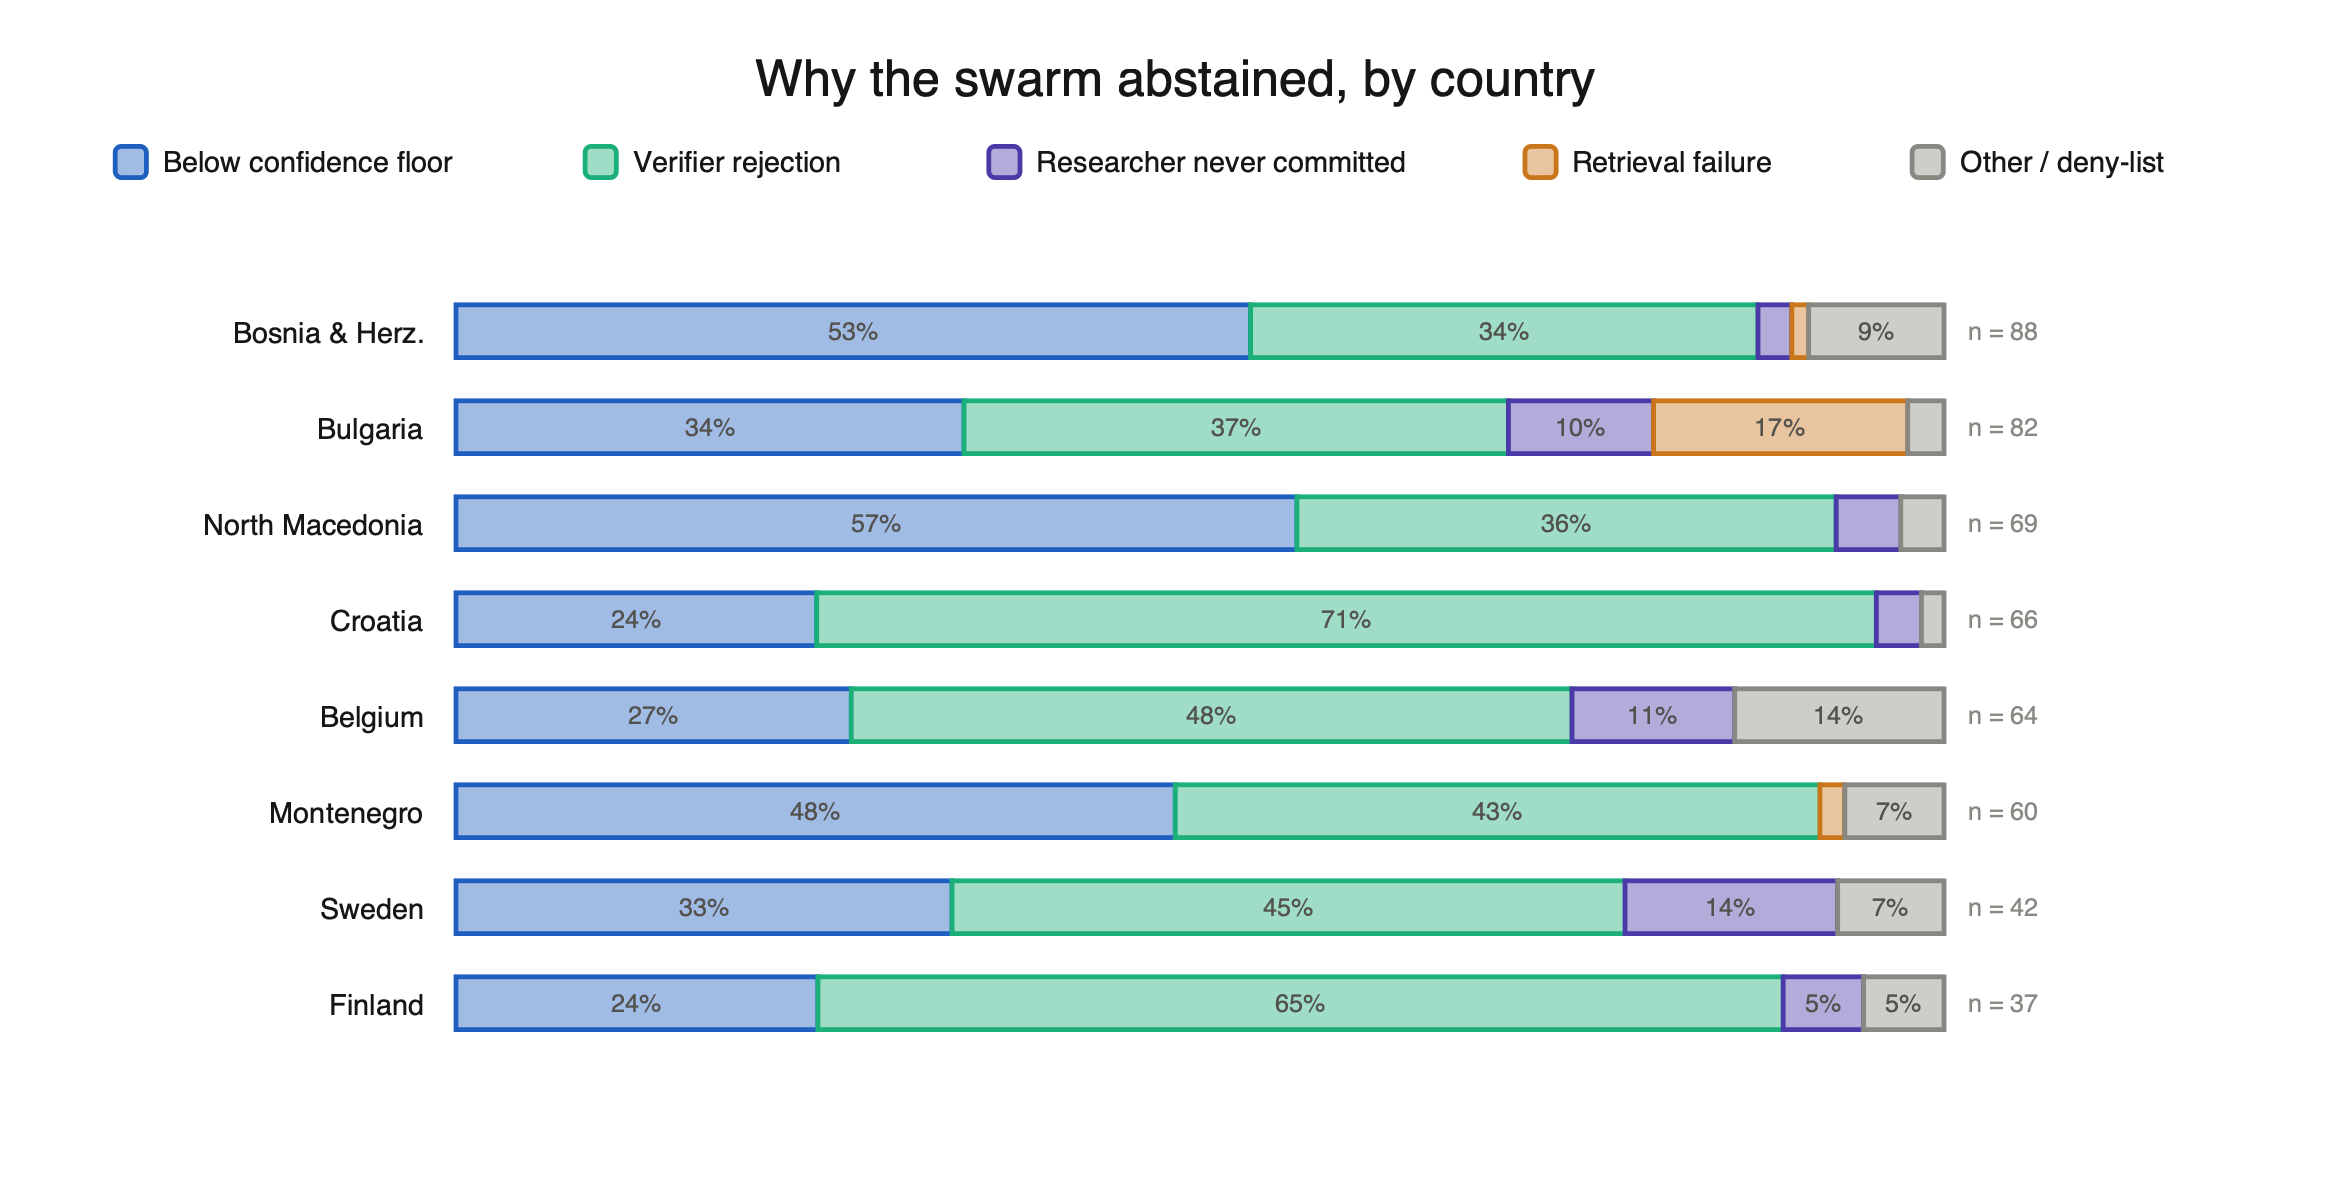
\includegraphics[width=6.1in,height=3.06297in]{media/media/image22.png}

@@CL@@Figure B.1: Why the swarm abstained, by country. The 508 evaluation abstentions grouped into five causes.@@/CL@@

\textbf{@@CL@@The quote citation gate, Attributability part 1@@/CL@@}

The gate is deliberately lenient, however, in three recorded ways. The comparison normalises Unicode and case, strips punctuation and collapses whitespace, and sets no minimum quote length, so a two- or three-word string or a light paraphrase satisfies it. The cited URL is checked only for membership of the result set, with nothing binding a quote to the page it was read on, so a passage from one page can be filed against another. Nothing compares the retrieved snippet against the live page, so where the picker has paraphrased, the gate certifies the paraphrase. The normalisation is deliberate as an exact byte comparison fails on encoding differences, smart quotes and whitespace artefacts that are not misquotes, and would discard correct answers. Quality assurance is the price of this.~So the worst case the gate lets through is a committed answer whose quote is real but thin, a handful of genuine words, or a paraphrase of them, that a reader would not accept as settling the question. It holds against fabrication and hands misattribution to the Verifier.

\textbf{@@CL@@The false-positive audit@@/CL@@}

@@CL@@Every committed answer that disagrees with a published ``no'' is a false positive, and the evaluation run produced 94 of them. The audit exists because a disagreement is not automatically a swarm error: the published answer is a country\textquotesingle s own self-report and can be a cycle out of date, so the question is whether the swarm over-read its evidence or found something the assessors missed. Each case was put to a separate reviewer, claude-opus-4-6, with the swarm\textquotesingle s own cited passage and the ODMI\textquotesingle s published explanation in front of it. 91 of the 94 are committed yes answers and were adjudicated; the remaining three, MK I4, Q5 and Q6, answer not applicable against a no gold, which the yes-defending rubric cannot score, so they are flagged for manual review rather than judged.@@/CL@@

The first framing is neutral. The reviewer is shown the ODMI gold answer and its published explanation and asked to account for the disagreement, with the prompt stating it must be ``strict and concrete''. Is this a genuine error, where the swarm misread evidence a reader would have rejected? A definitional gap, where the swarm answered a slightly different question than the one the ODMI scored? Or a defensible answer against a gold that may itself be stale or self-reported? The pass sorts the false positives by why they went wrong.

The second framing is pro-swarm. The reviewer is instructed to act as an advocate for swarm, being asked to build the ``strongest possible evidence-grounded case'' that the swarm\textquotesingle s ``yes'' was right and the ODMI\textquotesingle s ``no'' was mistaken, and to return one of three verdicts: that the swarm over-read its evidence even on the most generous reading, that the case is ambiguous, or that the gold is wrong and the swarm is vindicated. This is the stringent test. A false positive counts as the swarm being right only if a reviewer actively trying to prove that, from the evidence the swarm itself cited, can succeed.

{\def\LTcaptype{none} % do not increment counter
\begin{longtable}[]{@{}
  >{\raggedright\arraybackslash}p{(\linewidth - 6\tabcolsep) * \real{0.1671}}
  >{\raggedright\arraybackslash}p{(\linewidth - 6\tabcolsep) * \real{0.5504}}
  >{\raggedright\arraybackslash}p{(\linewidth - 6\tabcolsep) * \real{0.0688}}
  >{\raggedright\arraybackslash}p{(\linewidth - 6\tabcolsep) * \real{0.0885}}@{}}
\toprule\noalign{}
\begin{minipage}[b]{\linewidth}\raggedright
\textbf{@@CL@@Pass@@/CL@@}
\end{minipage} & \begin{minipage}[b]{\linewidth}\raggedright
\textbf{@@CL@@Verdict@@/CL@@}
\end{minipage} & \begin{minipage}[b]{\linewidth}\raggedright
\textbf{@@CL@@n@@/CL@@}
\end{minipage} & \begin{minipage}[b]{\linewidth}\raggedright
\textbf{@@CL@@Share@@/CL@@}
\end{minipage} \\
\midrule\noalign{}
\endhead
\bottomrule\noalign{}
\endlastfoot
@@CL@@Pass 1, charitable@@/CL@@ & @@CL@@Genuine error, the swarm misread evidence a reader would have rejected@@/CL@@ & @@CL@@16@@/CL@@ & @@CL@@18\%@@/CL@@ \\
& @@CL@@Definitional gap, the swarm answered a slightly different question@@/CL@@ & @@CL@@69@@/CL@@ & @@CL@@76\%@@/CL@@ \\
& @@CL@@Defensible, or the gold may be stale@@/CL@@ & @@CL@@6@@/CL@@ & @@CL@@7\%@@/CL@@ \\
@@CL@@Pass 2, advocate@@/CL@@ & @@CL@@Swarm over-read its evidence even on the most generous reading@@/CL@@ & @@CL@@68@@/CL@@ & @@CL@@75\%@@/CL@@ \\
& @@CL@@Ambiguous@@/CL@@ & @@CL@@23@@/CL@@ & @@CL@@25\%@@/CL@@ \\
& @@CL@@Gold wrong, swarm vindicated@@/CL@@ & @@CL@@0@@/CL@@ & @@CL@@0\%@@/CL@@ \\
\end{longtable}
}

@@CL@@Table B.2: The false-positive audit, over the 91 adjudicated cases of the 94. Shares are of 91.

The two passes agree on the direction. Nothing in the audit supports the swarm against the published key: the advocate pass returns ``no'' case at all where the gold is wrong and the swarm right. That is what licenses treating match against ODMI as a fair measure rather than one inflated by stale ground truth, and it is the basis for the staleness band §3.4 discusses being treated as negligible.@@/CL@@

\section{@@CC@@C. Experiments@@/CC@@}\label{ccc.-experimentscc}

@@CL@@Every experiment was registered before dispatch, in a design note fixing the question, the sample, the endpoint and the adoption rule, and in a machine-readable row carrying the same design. The table below is that register, filtered to the runs that completed. The paragraph after it is the model comparison, reproduced from §4.8 because the numbers behind it live in this appendix rather than in the body.@@/CL@@

\textbf{@@CL@@The completed experiments@@/CL@@}

\textbf{@@CL@@Model choice@@/CL@@}

Another lever on this cost is the choice of model, which sets both the reasoning model and the model that picks the snippets. Comparing models from the same family on the same 156 development-set pairs, Haiku 4.5 delivered 28.8\% accuracy, Sonnet 4.6 delivered 34.0\% at 1.4 times Haiku\textquotesingle s cost per correct answer, and Opus 4.8 delivered 21.8\% at 4.6 times. Opus is dominated on both axes, being the least accurate and the most expensive of the three. Coverage explains the ordering. Haiku committed to 43\% of the battery, Sonnet to 46.8\% and Opus to 29.5\%, and total accuracy counts an abstention as a failure. On committed answers alone the three converge, at 67.2\% for Haiku, 72.6\% for Sonnet and 73.9\% for Opus. With this lens Opus is not worse at answering these questions, it is more reluctant to answer them, and marginally the most accurate when it does. Like the Verifier stance in @@CL@@§4.7@@/CL@@, changing the model moves how much the system is willing to say rather than how often it is right. Sonnet is retained because it commits most, at a middling price, with commit-accuracy indistinguishable from a model costing over three times as much.

Completed experiments:

{\def\LTcaptype{none} % do not increment counter
\begin{longtable}[]{@{}
  >{\raggedright\arraybackslash}p{(\linewidth - 8\tabcolsep) * \real{0.1106}}
  >{\raggedright\arraybackslash}p{(\linewidth - 8\tabcolsep) * \real{0.2295}}
  >{\raggedright\arraybackslash}p{(\linewidth - 8\tabcolsep) * \real{0.2428}}
  >{\raggedright\arraybackslash}p{(\linewidth - 8\tabcolsep) * \real{0.2362}}
  >{\raggedright\arraybackslash}p{(\linewidth - 8\tabcolsep) * \real{0.1808}}@{}}
\toprule\noalign{}
\begin{minipage}[b]{\linewidth}\raggedright
\textbf{Exp}
\end{minipage} & \begin{minipage}[b]{\linewidth}\raggedright
\textbf{Experiment}
\end{minipage} & \begin{minipage}[b]{\linewidth}\raggedright
\textbf{Scope (n)}
\end{minipage} & \begin{minipage}[b]{\linewidth}\raggedright
\textbf{Result}
\end{minipage} & \begin{minipage}[b]{\linewidth}\raggedright
\textbf{Outcome}
\end{minipage} \\
\midrule\noalign{}
\endhead
\bottomrule\noalign{}
\endlastfoot
EXP-1 & Search provider: DIY vs Tavily & France, 90 pairs (55 decided) & DIY at least as good on 89\% of decided pairs (Wilson 78-95), leads all three dimensions & DIY adopted \\
EXP-17 & Snippet picker on vs off & Netherlands, n=50 & Recall unchanged; removing it raised cost \textasciitilde57\% and cut coverage & Keep the picker \\
EXP-17, EXP-18 & Retrieval breadth (5 vs 10 results) & Netherlands n=50; multi-country FR+AL+NL & The r10 gain rested on a single NL run at +17\% cost and never confirmed multi-country & Keep 5 results per query \\
EXP-24 & Snippet truncation cap & Netherlands replay, 25 abstained pairs & 3,000-char cap committed 15 vs 12 with no gain in correct answers and three abstain-to-wrong flips & Keep 600 \\
EXP-34 & Trusted-domain narrow-then-widen retrieval & NL+MT+AL, 156-pair dev battery & @@CC@@Clean null: pooled false-positive McNemar p = 0.727, paired accuracy an exact tie@@/CC@@ & @@CC@@No detectable difference@@/CC@@ \\
EXP-11 & Verifier redesign (tristate / gated) & Dev ladder, 150 frozen candidates & Incumbent disprove J = 0.41 against tristate 0.03 and the deterministic gate 0.02 & Retain incumbent \\
EXP-12 & Verifier evidence ladder & Dev + Malta / Norway & Counter-search helps no-claims, hurts yes-claims & Informs D45 \\
EXP-38 & Corroborative vs adversarial verifier framing & 150 frozen candidates, search-free replay & Disprove J = 0.41 against corroborate J = 0.16 via a sensitivity collapse 0.72 to 0.32; adversarialism costs twice the false-rejection rate & Adversarial framing retained; the trade reported \\
EXP-13a & Value of the verify-and-adjudicate layer & Malta 60 + Norway 143 & Removing it costs 27 correct and adds 43 abstentions & Keep the layer \\
EXP-14 & Verifier counter-search (never vs always) & Netherlands, n=51 & No significant difference (McNemar p = 0.50); \textquotesingle never\textquotesingle{} raises false positives & Keep \textquotesingle always\textquotesingle{} \\
EXP-19 & Verifier counter-search, multi-country & NL+MT+AL, \textasciitilde78 negative golds & Pooled marginal favours \textquotesingle never\textquotesingle{} but is composition-confounded; paired McNemar null (p = 1.00) & Keep \textquotesingle always\textquotesingle{} \\
EXP-16 & Adjudicator free vs standard selection & Netherlands, n=51 & No difference (p = 1.00) & Keep \textquotesingle standard\textquotesingle{} \\
EXP-7 & Retry chaining (carry evidence across retries) & Malta, 40 per arm & Small, underpowered gain; joint non-inferiority passes & Adopt as optimisation baseline \\
EXP-20 & Retry chaining on committing countries & NL+AL & Balanced accuracy rises but false-positive rate rose 0.346 to 0.387; McNemar p = 0.500 & Keep baseline; not promoted \\
EXP-10 & Confidence-floor sweep & Pooled, 7 countries, n=360, 67 negative golds & 0.65 holds; at 0.50 precision is 0.76, under the pre-registered 0.80 bar & Floor 0.65 \\
EXP-25, EXP-27 & Commit gates (entailment, argue-the-opposite) & Netherlands, n=50, 25 negative golds & Null and harmful; both raise the negative-gold false-positive rate & The 0.65 floor remains the precision control \\
EXP-22 & Foreign-language query ablation & Albania & Null: suppressing the native-language query changed nothing & Keep bilingual queries \\
EXP-39 & Language-comprehension probes (no DeepL) & Frozen 150 subset, local OPUS-MT & Part A null after the mandated translation-quality gate; third independent language null & No comprehension penalty demonstrated \\
EXP-32 & All-Haiku whole-stack cost point & 156-pair dev battery & Lower anchor of the cost-quality frontier & Frontier point, not adopted \\
EXP-41 & Run-to-run stability & 3 replicates, 148-pair intersection & Label agreement 0.922, three-way unanimity 0.703, evidence-path divergence 0.894 & Answers stable, evidence paths are not \\
EXP-36 & Frozen headline whole-system run & Evaluation 8, 1,144 pairs & Coverage 0.556, commit-accuracy 0.701 {[}0.664, 0.736{]}, negative-gold FPR 0.247, ECE 0.063 & The reported headline \\
EXP-28 & Architecture ablation ladder (researcher only / no adjudicator / trio). Sonnet 5, superseded by Table 4.7.1 & 156-pair dev battery, 78 negative golds & Commit rate 0.237, 0.391, 0.468 and commit-accuracy 0.649, 0.689, 0.726 across the three arms; negative-gold false-positive rate rises 0.13 to 0.22 (ten wrong to seventeen of 78) & Each layer adds coverage and accuracy; the Verifier does not filter for precision \\
EXP-40 & Corroborative vs adversarial verifier, end to end & 156-pair dev battery & Balanced accuracy 0.261 against 0.262; sixteen discordant pairs split eight-eight; McNemar p = 1.00 & Null end to end, against the EXP-38 frozen-ladder result \\
@@CC@@exp36\_model\_opus@@/CC@@ & @@CC@@All-Opus whole-stack cost point@@/CC@@ & @@CC@@156-pair dev battery@@/CC@@ & @@CC@@Delivered accuracy 21.8\% at £22.12, £0.65 per correct answer; worse than Sonnet 4.6 (p \textless{} 0.001) and Haiku 4.5 (p = 0.035)@@/CC@@ & @@CC@@Upper anchor of the cost-quality frontier; dominated on both axes, not adopted@@/CC@@ \\
@@CC@@cb\_heldout\_20260725@@/CC@@ & @@CC@@Closed-book parametric probe (retrieval disabled)@@/CC@@ & @@CC@@Evaluation 8, 1,144 pairs@@/CC@@ & @@CC@@42.9\% of the answer key reproduced against the 47.3\% always-yes floor@@/CC@@ & @@CC@@Below the floor; no answer-key memorisation demonstrated@@/CC@@ \\
@@CC@@heldout\_fp\_audit\_merged94@@/CC@@ & @@CC@@False-positive audit of the evaluation negative-gold errors@@/CC@@ & @@CC@@94 EXP-36 false positives, 91 adjudicable@@/CC@@ & @@CC@@Charitable pass: 16/91 genuine swarm error, 69/91 definitional gap, 6/91 defensible or stale gold. Adversarial pass: 0/91 gold wrong@@/CC@@ & @@CC@@No case of the swarm right and ODMI wrong; the 3 not\_applicable pairs flagged for manual review@@/CC@@ \\
\end{longtable}
}

@@CL@@Table C.1: The completed experiments, with the sample, result and adoption rule for each.@@/CL@@

\textbf{@@CL@@What the orchestrator refuses@@/CL@@}

@@CC@@The orchestrator refuses to dispatch a run where the experiment identifier has no row in the registry, where two arms differ from the baseline in more than one setting, where a specification names an evaluation country, where two arms share an identifier, or where no ceiling has been declared on the number of model calls the run may spend. Each is a hard failure that halts the run before any expenditure.@@/CC@@

\section{D. Out-of-Reach Questions}\label{d.-out-of-reach-questions}

@@CC@@The 29 questions judged systematically out of reach of a web agent. The rule is that the answer is a fact about internal operational behaviour for which there is no standard public artefact. Questions answerable from a policy document, observable as a portal feature, computable from harvested metadata, or which themselves ask whether something is published, are excluded. The classification was made from the question text alone, before any run data was consulted.@@/CC@@

{\def\LTcaptype{none} % do not increment counter
\begin{longtable}[]{@{}
  >{\raggedright\arraybackslash}p{(\linewidth - 2\tabcolsep) * \real{0.1386}}
  >{\raggedright\arraybackslash}p{(\linewidth - 2\tabcolsep) * \real{0.8614}}@{}}
\toprule\noalign{}
\begin{minipage}[b]{\linewidth}\raggedright
\textbf{Question}
\end{minipage} & \begin{minipage}[b]{\linewidth}\raggedright
\textbf{Text}
\end{minipage} \\
\midrule\noalign{}
\endhead
\bottomrule\noalign{}
\endlastfoot
P18 & Is there a regular exchange of knowledge or experiences between the national open data team and the team maintaining the national portal? \\
P20 & Is there a regular exchange of knowledge or experiences between the national open data team and the wider network of open data officers in your country? \\
P25 & Are there any processes in place to assess if public sector bodies are charging for data above marginal cost? (please see directive (EU) 2019/1024 on open data and the reuse of public sector information). \\
PT15 & Does the team monitor the extent to which requests (either via the portal or otherwise) result in the publication of the requested data? \\
PT23 & Do you monitor the portal\textquotesingle s traffic (e.g. in terms of number of unique visitors, visitor profiles, percentage of machine traffic, number of downloads according to the number of datasets etc.)? \\
PT24 & Do you run analytics on API usage? \\
PT25 & Besides monitoring portal traffic, do you perform any further activities to better understand the behaviour and needs of users of your portal (e.g. web analytics, surveys, or analysis of social media feeds)? \\
PT26 & Do you use the insights about portal usage and about the behaviour and needs of portal users to improve the portal accordingly? \\
PT28 & Do you monitor what keywords are used to search for data and content on the portal? \\
PT29 & Do you monitor the most and least consulted pages? \\
PT33 & Do you identify the data providers that are not yet publishing data on the national portal? \\
PT34 & Were there concrete actions taken to assist these data providers with their publication process? \\
PT44 & Do you monitor the characteristics of the data published on the portal, such as the distribution across categories, static vs. real-time data and how these change over time? \\
PT45 & Does this monitoring enable the portal team and/or data providers to take action to improve their performance on the national portal? \\
Q1 & Is there a pre-defined approach to ensure that metadata is kept up-to-date? \\
Q4 & Do you undertake efforts to ensure that published data covers the full period from when it was first published until today, for example, the complete time series? \\
Q7 & Do you monitor the quality of the metadata available on your portal? \\
Q20 & Do you investigate the most common causes for the lack of DCAT-AP compliance? \\
I4 & Does your country have processes in place to monitor and measure the level of reuse of high-value datasets ((EU) 2023/138)? \\
I8 & Have any public bodies in your country launched or performed any activities in the past year to understand which and how (open) datasets are reused? \\
I8-a & Automated feedback mechanisms tracking users´ access to datasets \\
I8-b & Surveys \\
I8-c & Interviews/workshops with reusers \\
I8-d & Other \\
I9 & Have any public bodies in your country launched or performed any activities in the past year to better understand reusers\textquotesingle{} needs in order to further stimulate the reuse of open data? \\
I9-a & Regular feedback sessions with portal users \\
I9-b & Social media sentiment analysis \\
I9-c & Other \\
I11 & Are there any public bodies in your country that have developed a systematic ways of classifying the gathered reuse cases? \\
\end{longtable}
}

@@CL@@Table D.1: The 29 questions judged out of reach of a web agent.@@/CL@@

\section{@@CC@@E. Prior Work Scored Against the Six Criteria, with Justifications@@/CC@@}\label{cce.-prior-work-scored-against-the-six-criteria-with-justificationscc}

@@CC@@The abridged version of this table@@/CC@@@@CL@@, Table E.1,@@/CL@@@@CC@@ appears as Table 2.2@@/CC@@@@CL@@ in §2.8@@/CL@@@@CC@@. Verdicts are read from the papers themselves, and quoted passages are taken verbatim from the primary text. A tick means the work addresses and reports the criterion, not that it succeeds. Partial means it addresses one of the criterion's two conditions, or reports it without measuring it.@@/CC@@

{\def\LTcaptype{none} % do not increment counter
\begin{longtable}[]{@{}
  >{\raggedright\arraybackslash}p{(\linewidth - 12\tabcolsep) * \real{0.1427}}
  >{\raggedright\arraybackslash}p{(\linewidth - 12\tabcolsep) * \real{0.1428}}
  >{\raggedright\arraybackslash}p{(\linewidth - 12\tabcolsep) * \real{0.1429}}
  >{\raggedright\arraybackslash}p{(\linewidth - 12\tabcolsep) * \real{0.1427}}
  >{\raggedright\arraybackslash}p{(\linewidth - 12\tabcolsep) * \real{0.1428}}
  >{\raggedright\arraybackslash}p{(\linewidth - 12\tabcolsep) * \real{0.1430}}
  >{\raggedright\arraybackslash}p{(\linewidth - 12\tabcolsep) * \real{0.1429}}@{}}
\toprule\noalign{}
\begin{minipage}[b]{\linewidth}\raggedright
@@CC@@Work@@/CC@@
\end{minipage} & \begin{minipage}[b]{\linewidth}\raggedright
@@CC@@Convergent Validity@@/CC@@
\end{minipage} & \begin{minipage}[b]{\linewidth}\raggedright
@@CC@@Generalisability@@/CC@@
\end{minipage} & \begin{minipage}[b]{\linewidth}\raggedright
@@CC@@Subgroup Equity@@/CC@@
\end{minipage} & \begin{minipage}[b]{\linewidth}\raggedright
@@CC@@Attributability@@/CC@@
\end{minipage} & \begin{minipage}[b]{\linewidth}\raggedright
@@CC@@Selectivity@@/CC@@
\end{minipage} & \begin{minipage}[b]{\linewidth}\raggedright
@@CC@@Reproducibility@@/CC@@
\end{minipage} \\
\midrule\noalign{}
\endhead
\bottomrule\noalign{}
\endlastfoot
@@CC@@ReAct (Yao et al., 2023)@@/CC@@ & @@CC@@Reports accuracy on HotpotQA and Fever and success-rate gains of 34\% and 10\% on ALFWorld and WebShop, against task gold rather than a human assessor key.@@/CC@@ & @@CC@@Four benchmarks over two families, question answering and interactive decision making.@@/CC@@ & @@CC@@Not addressed.@@/CC@@ & @@CC@@Retrieves through "a simple Wikipedia API" and leaves trajectories "more interpretable than baselines without reasoning traces". No check that a quoted passage exists in the source.@@/CC@@ & @@CC@@No abstention and no confidence output.@@/CC@@ & @@CC@@"All methods use greedy decoding" and prompts are published. No repeated runs and no variance.@@/CC@@ \\
@@CC@@SelfCheckGPT (Manakul et al., 2023)@@/CC@@ & @@CC@@AUC-PR against manual factuality annotation. No agreement percentage reported.@@/CC@@ & @@CC@@WikiBio only, with synthetically generated hallucinations.@@/CC@@ & @@CC@@Not addressed.@@/CC@@ & @@CC@@Zero-resource by design. External knowledge appears only as an ablation showing what could be done instead.@@/CC@@ & @@CC@@Produces a per-sentence hallucination score that could drive a gate, but never declines and reports no calibration.@@/CC@@ & @@CC@@Main response at "temperature to 0.0 and standard beam search decoding". Sampling is internal to the method and is not a stability measure.@@/CC@@ \\
@@CC@@Chain-of-Verification (Dhuliawala et al., 2024)@@/CC@@ & @@CC@@Reports hallucination reduction across tasks with no single headline agreement figure.@@/CC@@ & @@CC@@Three task types, Wikidata list questions, closed-book MultiSpanQA and long-form generation.@@/CC@@ & @@CC@@Not addressed.@@/CC@@ & @@CC@@Tool-free by design. Retrieval appears only as related work.@@/CC@@ & @@CC@@No abstention and no confidence. Confidence scoring is attributed to Varshney et al., not to CoVe.@@/CC@@ & @@CC@@"Use greedy decoding for all models". No repeated runs.@@/CC@@ \\
@@CC@@LM vs LM (Cohen et al., 2023)@@/CC@@ & @@CC@@"Detects over 70\% of the incorrect claims while maintaining a high precision".@@/CC@@ & @@CC@@Four benchmarks.@@/CC@@ & @@CC@@Not addressed.@@/CC@@ & @@CC@@"We are not assuming any reference text or an external knowledge base." The examiner asks whether external evidence exists without ever retrieving any.@@/CC@@ & @@CC@@Frames its setting as related to calibration and abstention, but outputs a decision and never declines.@@/CC@@ & @@CC@@Applies the method "three times (with the same EXAMINER and EXAMINEE), using sampling" for the majority variant.@@/CC@@ \\
@@CC@@Du et al. (2023)@@/CC@@ & @@CC@@Accuracy across six benchmarks against task gold.@@/CC@@ & @@CC@@Six benchmarks including mathematics, MMLU and chess move validity.@@/CC@@ & @@CC@@Not addressed.@@/CC@@ & @@CC@@Retrieval is described as orthogonal to the method and is not used.@@/CC@@ & @@CC@@Observes that uncertain facts diverge across agents, but provides no abstention channel.@@/CC@@ & @@CC@@Reports standard deviations throughout, for example "Single Agent 67.0 ± 4.7" and "Multi-Agent (Majority) 69.0 ± 4.6", with identical prompt and model across arms.@@/CC@@ \\
@@CC@@Liang et al. (2023)@@/CC@@ & @@CC@@Reports gains on two datasets against task gold.@@/CC@@ & @@CC@@Two datasets, commonsense machine translation and counter-intuitive arithmetic reasoning.@@/CC@@ & @@CC@@Not addressed.@@/CC@@ & @@CC@@No retrieval.@@/CC@@ & @@CC@@No abstention and no confidence.@@/CC@@ & @@CC@@"Experiments are performed in zero-shot instructions (setting temperature to 0)". Deterministic and traceable, with no stability measure.@@/CC@@ \\
@@CC@@Smit et al. (2024)@@/CC@@ & @@CC@@Reports a state-of-the-art MedQA result for GPT-3.@@/CC@@ & @@CC@@Multiple-choice questions "across a wide range of domains", MedQA foremost.@@/CC@@ & @@CC@@Not addressed.@@/CC@@ & @@CC@@No retrieval or evidence grounding.@@/CC@@ & @@CC@@No abstention and no confidence.@@/CC@@ & @@CC@@"Analyze the top three runs for each system", with an open-source repository and evaluation scripts released.@@/CC@@ \\
@@CC@@Zhu et al. (2026)@@/CC@@ & @@CC@@Outperforms vanilla debate and majority vote across six benchmarks.@@/CC@@ & @@CC@@Six reasoning-oriented QA benchmarks.@@/CC@@ & @@CC@@Not addressed.@@/CC@@ & @@CC@@No retrieval or evidence grounding.@@/CC@@ & @@CC@@Central to the paper. Agents "express calibrated confidence and condition their updates on others' confidence", but the system never declines.@@/CC@@ & @@CC@@Reports 95\% confidence intervals and a full hyperparameter table.@@/CC@@ \\
@@CC@@SAFE (Wei et al., 2024)@@/CC@@ & @@CC@@"SAFE agrees with crowdsourced human annotators 72\% of the time" over 16,011 individual facts, and wins 76\% of a 100-case disagreement sample.@@/CC@@ & @@CC@@LongFact, "2,280 fact-seeking prompts across 38 manually-selected topics", over 13 models in 4 families.@@/CC@@ & @@CC@@Not addressed. Apparent mentions are a question topic and a boilerplate ethics statement.@@/CC@@ & @@CC@@Google Search per claim, with each atomic fact rated against the retrieved results.@@/CC@@ & @@CC@@Three-way output of Supported, Not Supported and Irrelevant, so a third state exists, but there is no confidence score and no calibration.@@/CC@@ & @@CC@@"gpt-4-0613 at a temperature of 1.0", with model versions named. Metrics are "averaged over 250 evaluation examples", so over examples and not over runs.@@/CC@@ \\
@@CC@@Feng et al. (2024)@@/CC@@ & @@CC@@Up to 19.3\% improvement in abstain accuracy over the strongest baseline, reported as R-Acc, ER, A-Acc and A-F1.@@/CC@@ & @@CC@@Four datasets and three LLMs, plus the curated ElectionQA23.@@/CC@@ & @@CC@@The only prior work to measure it. Splits ElectionQA23 by continent and finds "LLMs' abstain rate is often lower for elections in Africa and Asia, shedding light on the potential fairness issues in LLM abstention".@@/CC@@ & @@CC@@Analyses failure cases in retrieval augmentation, but the abstention methods themselves probe knowledge gaps rather than cite sources.@@/CC@@ & @@CC@@The subject of the paper. Calibration, training, prompting, consistency and collaboration strategies for abstention, with abstain ECE reported.@@/CC@@ & @@CC@@"Sampling temperature to 0.1, and 0.7 where employing an LLM as the final judge to decide multiple runs are required".@@/CC@@ \\
@@CC@@Chowdhury et al. (2026)@@/CC@@ & @@CC@@81.7\% on Check-COVID, against 85.8\% for a single-call GPT-5-mini with RAG and 71.7\% for standard multi-agent debate.@@/CC@@ & @@CC@@Check-COVID at 120 claims, HealthVer at 100 and 78.3\% on FEVEROUS at 60, though Table 7 is captioned "Generalization results (single run)".@@/CC@@ & @@CC@@Not addressed.@@/CC@@ & @@CC@@Progressive RAG with evidence admission protocols, expanding the evidence pool during the debate.@@/CC@@ & @@CC@@An INCONCLUSIVE verdict, a computed confidence score, and an ECE of 0.034 after tuning judge weights by 5-fold cross-validation.@@/CC@@ & @@CC@@The only prior work to measure stability. "Table 3 reports Check-COVID performance across three independent runs", and the limitations concede "run-level variance remains notable despite majority voting".@@/CC@@ \\
@@CC@@Fumega and Gao (2026)@@/CC@@ & @@CC@@An ``average mismatch rate of 42\% between the AI's answers and those of human researchers'' across four indicators in their end-to-end phase.@@/CC@@ & @@CC@@By indicator, mismatch of 19\% on Data Protection (2 of 12 questions) against 69\% on Land Tenure (17 of 25), chosen respectively for single-document and fragmented evidence. Their stated percentages do not reconcile with their own counts.@@/CC@@ & @@CC@@Not addressed. The sample is drawn from Africa and Latin America, but results are not broken down by region.@@/CC@@ & @@CC@@The agents are prompted for ``justifications (with a link to the evidence)'' per sub-question, so a trail exists, but nothing checks that the link supports the claim. Both reported failures are of that kind, an ``API Access'' button cited as evidence of bulk access, and ``corporate body'' read as covering group privacy.@@/CC@@ & @@CC@@No abstention. "Partially" is an answer option and not a decline, and uncertainty calibration appears only in the future-work list. Incompleteness is handled by "a human-in-the-loop approach for curation and validation".@@/CC@@ & @@CC@@Table 2 documents tools and configuration by phase, but no run is repeated and no variance is reported.@@/CC@@ \\
@@CC@@This work@@/CC@@ & @@CC@@Tested against the human key and against an independent deterministic recompute.@@/CC@@ & @@CC@@Decomposed by ODMI dimension and by question form.@@/CC@@ & @@CC@@Decomposed by language-resource stratum.@@/CC@@ & @@CC@@Offline quote-in-source gate on every committed answer, plus Verifier entailment judgement.@@/CC@@ & @@CC@@Three-way outcome with a confidence floor driving abstention, calibration assessed post-hoc.@@/CC@@ & @@CC@@Full transcript logging, with stability measured across repeated runs.@@/CC@@ \\
\end{longtable}
}

@@CC@@Table E.1: Prior work scored against the six criteria of §2.2, with the evidence for each verdict.@@/CC@@

\section{@@CL@@F. Baselines@@/CL@@}\label{clf.-baselinescl}

@@CL@@The baselines the evaluation results are read against. @@/CL@@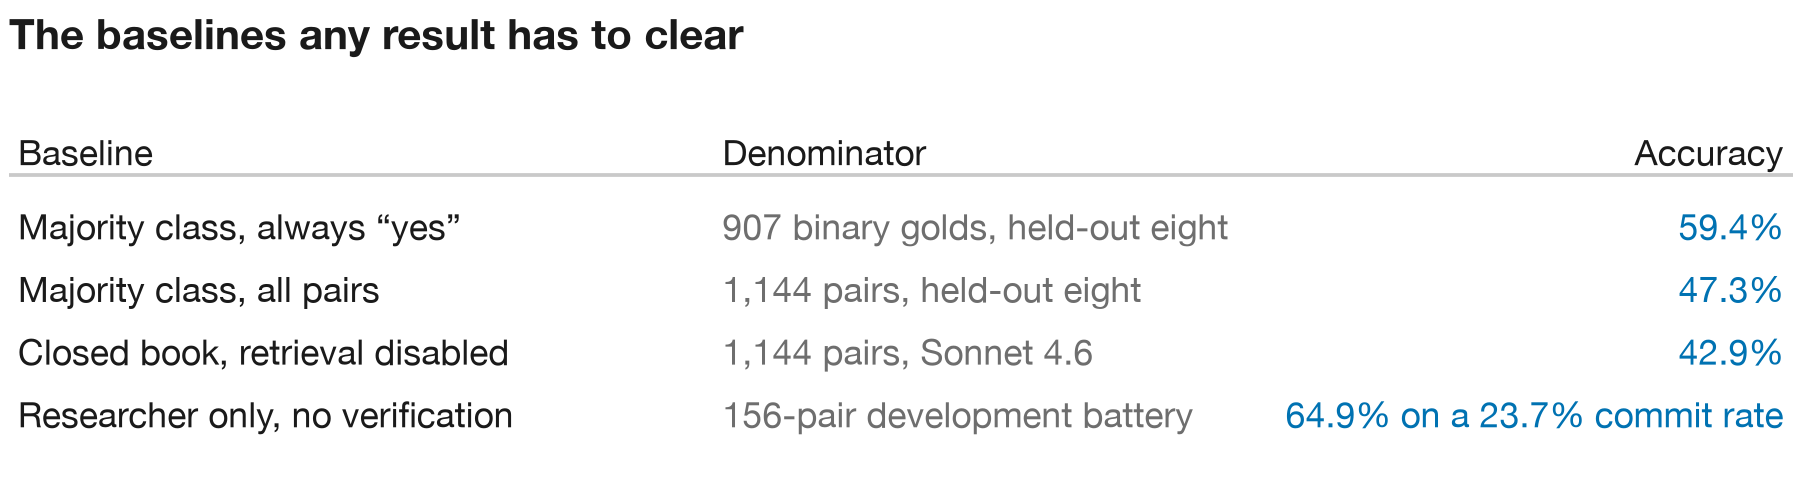
\includegraphics[width=6.1in,height=1.67996in]{media/media/image23.png}

@@CL@@Table F.1: The baselines any result has to clear.@@/CL@@\textbf{@@CC@@ @@/CC@@}

{\def\LTcaptype{none} % do not increment counter
\begin{longtable}[]{@{}
  >{\raggedright\arraybackslash}p{(\linewidth - 6\tabcolsep) * \real{0.2157}}
  >{\raggedright\arraybackslash}p{(\linewidth - 6\tabcolsep) * \real{0.3039}}
  >{\raggedright\arraybackslash}p{(\linewidth - 6\tabcolsep) * \real{0.2059}}
  >{\raggedright\arraybackslash}p{(\linewidth - 6\tabcolsep) * \real{0.2745}}@{}}
\toprule\noalign{}
\begin{minipage}[b]{\linewidth}\raggedright
\textbf{Baseline}
\end{minipage} & \begin{minipage}[b]{\linewidth}\raggedright
\textbf{What it isolates}
\end{minipage} & \begin{minipage}[b]{\linewidth}\raggedright
\textbf{Value}
\end{minipage} & \begin{minipage}[b]{\linewidth}\raggedright
\textbf{Denominator}
\end{minipage} \\
\midrule\noalign{}
\endhead
\bottomrule\noalign{}
\endlastfoot
@@CC@@Always-yes, all 36 countries@@/CC@@ & @@CC@@what no reasoning at all scores on the full assessment@@/CC@@ & @@CC@@81.8\%@@/CC@@ & @@CC@@4,146 binary golds@@/CC@@ \\
@@CC@@Always-yes, evaluation eight@@/CC@@ & @@CC@@the same, once negative golds are oversampled@@/CC@@ & @@CC@@59.4\%@@/CC@@ & @@CC@@907 binary golds@@/CC@@ \\
@@CC@@Majority class, development battery@@/CC@@ & @@CC@@the same, on the class-balanced tuning set@@/CC@@ & @@CC@@50.6\%@@/CC@@ & @@CC@@154 binary golds; the majority class here is no, not yes@@/CC@@ \\
@@CC@@Closed-book, retrieval disabled@@/CC@@ & @@CC@@how much of the answer key the model already carries@@/CC@@ & @@CC@@42.9\%, against a 47.3\% floor@@/CC@@ & @@CC@@1,139 evaluation pairs@@/CC@@ \\
@@CC@@Researcher alone, no verification@@/CC@@ & @@CC@@what one agent reaches before any checking@@/CC@@ & @@CC@@23.7\% coverage, 64.9\% commit-accuracy@@/CC@@ & @@CC@@156-pair development battery, Sonnet 4.6@@/CC@@ \\
\end{longtable}
}

\section{@@CL@@G. The Full Question Bank@@/CL@@}\label{clg.-the-full-question-bankcl}

@@CL@@The complete ODMI questionnaire as the swarm sees it, all 143 questions in the order they appear in the instrument. This is the population every figure in Chapter 4 is drawn from, so it is here in full rather than sampled. By dimension: Policy 31, Portal 45, Quality 29 and Impact 38. By answer shape: 124 binary, 12 percentage bands, 3 ordinal magnitudes, 2 count bands and 2 categorical. The 124 binary questions are the ones the headline accuracy figures are computed over, because they are the only shape where a ``yes'' or ``no'' can be scored against the published key without a banding judgement.@@/CL@@

{\def\LTcaptype{none} % do not increment counter
\begin{longtable}[]{@{}
  >{\raggedright\arraybackslash}p{(\linewidth - 2\tabcolsep) * \real{0.1386}}
  >{\raggedright\arraybackslash}p{(\linewidth - 2\tabcolsep) * \real{0.8614}}@{}}
\toprule\noalign{}
\begin{minipage}[b]{\linewidth}\raggedright
\textbf{@@CL@@Question@@/CL@@}
\end{minipage} & \begin{minipage}[b]{\linewidth}\raggedright
\textbf{@@CL@@Text@@/CL@@}
\end{minipage} \\
\midrule\noalign{}
\endhead
\bottomrule\noalign{}
\endlastfoot
@@CL@@P1@@/CL@@ & @@CL@@Is there a national open data policy in your country and, if your country is an EU Member State, does this include a national legislation for the transposition of the Open Data Directive? For Explanation: * If yes, please provide (1) the URL and (2) title of the policy document and (3) briefly describe. * If `other', please provide (1) a brief explanation to support your answer choice and (2) provide the URL and indicate the policy section which explicitly references open data.@@/CL@@ \\
@@CL@@P2@@/CL@@ & @@CL@@Is there a national open data strategy in your country? For Explanation: * If yes, please provide (1) the URL to the strategy and (2) describe the main highlights. * If \textquotesingle not applicable\textquotesingle, please provide (1) a brief explanation to support your answer choice and provide (2) the URL and indicate the policy section which explicitly references objectives, actions/measures, delivery timelines etc.@@/CL@@ \\
@@CL@@P3@@/CL@@ & @@CL@@Is there an open data policy/strategy at regional or local level? For Explanation: * If yes, please (1) provide the URL and (2) title of the document(s) and (3) briefly describe.@@/CL@@ \\
@@CL@@P4@@/CL@@ & @@CL@@Does the national strategy/policy include an action plan with measures to be implemented in the open data field? For Explanation: If yes, please briefly describe the main measures described by the action plan.@@/CL@@ \\
@@CL@@P5@@/CL@@ & @@CL@@Does the national strategy/policy outline measures to incentivise the publication of and access to real-time or dynamic data? For Explanation: * If yes, please briefly describe the measures.@@/CL@@ \\
@@CL@@P6@@/CL@@ & @@CL@@Does the national strategy/policy outline measures to incentivise the publication of and access to citizen-generated data? For Explanation: * If yes, please briefly describe the measures.@@/CL@@ \\
@@CL@@P7@@/CL@@ & @@CL@@Does the national strategy/policy foster the discoverability of the aforementioned types of data from your country on data.europa.eu? For Explanation: * If yes, please briefly describe how.@@/CL@@ \\
@@CL@@P8@@/CL@@ & @@CL@@Does the national strategy/policy outline measures to support the reuse of open data by the public sector? For Explanation: * If yes, please briefly describe the measures.@@/CL@@ \\
@@CL@@P9@@/CL@@ & @@CL@@Does the national strategy/policy outline measures to support the reuse of open data by the private sector? For Explanation: * If yes, please briefly describe the measures.@@/CL@@ \\
@@CL@@P10-a@@/CL@@ & @@CL@@Does the national strategy/policy mandate carrying out and maintaining a data inventory by public bodies, whether at national or local level? For Explanation: * If yes, please briefly specify.@@/CL@@ \\
@@CL@@P10-b@@/CL@@ & @@CL@@Do these data inventories include the data collected by public bodies that cannot be published as open data (e.g. in relation to the EU Data Governance Act (EU) 2022/868)? For Explanation: * If yes, please briefly specify.@@/CL@@ \\
@@CL@@P11@@/CL@@ & @@CL@@Is your country applying the implementing regulation (EU) 2023/138 on high-value datasets? For Explanation: * If yes, how is it progressing? * If you are an EFTA or a candidate country to the EU, please select \textquotesingle not applicable\textquotesingle. ** In the table below, please indicate your progress with respect to a) organisation, b) legal aspects, c) technical aspects on a scale from 1 to 5. 1 = no progress; 2 = few progress; 3 = some progress; 4 = considerable progress; 5 = works are finalised.@@/CL@@ \\
@@CL@@P12@@/CL@@ & @@CL@@Have the public bodies in your country denoted relevant datasets as high-value datasets in their metadata following the publication of the implementing regulation (EU) 2023/138 on high-value datasets? For Explanation: * If yes, please specify how and highlight challenges, if any. * If you are an EFTA or a candidate country to the EU, please select \textquotesingle not applicable\textquotesingle.@@/CL@@ \\
@@CL@@P13@@/CL@@ & @@CL@@Is there a governance structure in place that enables the participation and/or inclusion of various open data stakeholders? For Explanation: * If yes, please briefly describe the governance structure and its operating model@@/CL@@ \\
@@CL@@P14@@/CL@@ & @@CL@@How would you classify the model used for governing open data in your country? For Explanation: * Please briefly explain why this model was chosen/works best for your country@@/CL@@ \\
@@CL@@P15@@/CL@@ & @@CL@@Does the governance structure ensure that the local and regional open data initiatives are facilitated and supported at national level? For Explanation: * If yes, please give an example of what kind of support. * If not applicable, please explain why.@@/CL@@ \\
@@CL@@P16@@/CL@@ & @@CL@@To what degree do local/regional public bodies conduct open data initiatives? For Explanation: * If not applicable, please explain why.@@/CL@@ \\
@@CL@@P17@@/CL@@ & @@CL@@Is a document describing the responsibilities and governance structure of the national (and/or regional/local) open data team publicly available? For Explanation: * If yes, please provide the URL where this information is published.@@/CL@@ \\
@@CL@@P18@@/CL@@ & @@CL@@Is there a regular exchange of knowledge or experiences between the national open data team and the team maintaining the national portal? For Explanation: * If yes, please briefly describe how this exchange takes place and provide evidence supporting your answer (e.g. meeting agendas, URLs to news items).@@/CL@@ \\
@@CL@@P19@@/CL@@ & @@CL@@Does the governance model include the appointment of official roles in civil services that are dedicated to open data (e.g. open data officers)? For Explanation: * If yes, please describe how this task is fulfilled at public body level.@@/CL@@ \\
@@CL@@P20@@/CL@@ & @@CL@@Is there a regular exchange of knowledge or experiences between the national open data team and the wider network of open data officers in your country? For Explanation: * If yes, please briefly describe how this exchange takes place and provide evidence supporting your answer (e.g. meeting agendas, URLs to news items).@@/CL@@ \\
@@CL@@P21@@/CL@@ & @@CL@@Is there a regular exchange of knowledge or experiences between public sector bodies (i.e. the providers) and open data reusers (e.g. academia, citizens, businesses)? For Explanation: * If yes, please briefly describe how this exchange takes place and provide evidence supporting your answer (e.g. meeting agendas, URLs to news items).@@/CL@@ \\
@@CL@@P22@@/CL@@ & @@CL@@Do data publication plans exist at public body level? For Explanation: * If yes, please provide the URL and briefly highlight the key aspects covered.@@/CL@@ \\
@@CL@@P23@@/CL@@ & @@CL@@Are there processes to ensure that the open data policies/strategy previously mentioned are implemented (e.g. monitoring)? For Explanation: * If yes, please specify the process(es).@@/CL@@ \\
@@CL@@P24@@/CL@@ & @@CL@@Are there processes to ensure that the open data policies/strategy previously mentioned are updated and revised as needed? For explanation: * If yes, please describe the process and any recent updates made to strategy/policy@@/CL@@ \\
@@CL@@P25@@/CL@@ & @@CL@@Are there any processes in place to assess if public sector bodies are charging for data above marginal cost? (please see directive (EU) 2019/1024 on open data and the reuse of public sector information). For Explanation: * If yes, please specify the process(es).@@/CL@@ \\
@@CL@@P26-a@@/CL@@ & @@CL@@What are the top 3 challenges that your country is facing in the implementation of the mentioned open data policies/strategy? For Explanation: * Please briefly describe.@@/CL@@ \\
@@CL@@P26-b@@/CL@@ & @@CL@@Are there activities in place to address these challenges in your country (e.g. with specific national/regional/local plans or initiatives)? For Explanation: * If yes, please briefly describe the measures that you have adopted or plan to adopt to address these challenges. * If no, please specify what is hampering finding a strategic approach to solve these challenges.@@/CL@@ \\
@@CL@@P27@@/CL@@ & @@CL@@Are there any activities in place to assist data holders with publishing their data as open data (i.e. to help them with the data opening process)? For Explanation: * If yes, please describe/provide examples of these activities.@@/CL@@ \\
@@CL@@P28@@/CL@@ & @@CL@@Is there a professional development or training plan for civil servants working with data in your country? For Explanation: * If yes, please briefly describe these training activities.@@/CL@@ \\
@@CL@@P29@@/CL@@ & @@CL@@Are there annually held national, regional or local events (e.g. hackathons, courses, conferences, users meet-ups, summer/winter schools) to promote open data and open data literacy in your country beyond the target group of public servants? For Explanation: * If yes, please provide examples (e.g. title, date, location of the event and URL).@@/CL@@ \\
@@CL@@PT1@@/CL@@ & @@CL@@Is there a national portal in your country for that enables users to search for open datasets and find where to download open data? For Explanation: * If yes, please provide the URL of the national portal.@@/CL@@ \\
@@CL@@PT2@@/CL@@ & @@CL@@For Explanation: * What is the technology stack of your portal (e.g. based on uData, CKAN, etc.)@@/CL@@ \\
@@CL@@PT3@@/CL@@ & @@CL@@Does the national portal offer to its users a way to programmatically query the metadata via an API? For Explanation: * If yes, please provide the direct-URL to this feature.@@/CL@@ \\
@@CL@@PT4@@/CL@@ & @@CL@@Does the national portal offer to its users a way to programmatically query the metadata via a SPARQL access point? For Explanation: * If yes, please provide the direct-URL to this feature.@@/CL@@ \\
@@CL@@PT5@@/CL@@ & @@CL@@Does the national portal offer/link to documentation on the use of APIs? For Explanation: * If yes, please provide the direct-URL to this feature.@@/CL@@ \\
@@CL@@PT6@@/CL@@ & @@CL@@Does the national portal offer/link to documentation on the use of SPARQL? For Explanation: * If yes, please provide the direct-URL to this feature.@@/CL@@ \\
@@CL@@PT7@@/CL@@ & @@CL@@Does the national portal provide functionality for users to contribute datasets they have produced or enriched? For explanation: * If yes, please (1) explain how the portal facilitate the linking of documentation and supporting materials to these user-contributed datasets and (2) provide the direct-URL to this feature.@@/CL@@ \\
@@CL@@PT8@@/CL@@ & @@CL@@Does the national portal offer a mechanism for users to provide general feedback, such a \textquotesingle Contact us\textquotesingle{} or \textquotesingle Feedback\textquotesingle{} button that is placed in a visible spot and would allows users to send a general comment concerning the portal? For Explanation: * If yes, please provide the direct-URL to this feature or describe how this functionality is provided.@@/CL@@ \\
@@CL@@PT9@@/CL@@ & @@CL@@Does the national portal offer a mechanism for users to provide feedback on specific datasets, such as a \textquotesingle feedback button\textquotesingle{} or a comment/discussion section under the dataset? For Explanation: * If yes, please provide the direct-URL to this feature or describe how this functionality is provided.@@/CL@@ \\
@@CL@@PT10@@/CL@@ & @@CL@@Does the national portal provide a mechanism for users to rate datasets? For Explanation: * If yes, please provide the direct-URL to this feature or describe how this functionality is provided.@@/CL@@ \\
@@CL@@PT11@@/CL@@ & @@CL@@Does the national portal enable users to find information and news on relevant open data topics in the country? For Explanation: * If yes, please provide the direct-URL to this feature.@@/CL@@ \\
@@CL@@PT12@@/CL@@ & @@CL@@Does the national portal offer the possibility for users to receive notifications when new datasets are available on the national portal (RSS, ATOM feeds, email notifications etc.)? For Explanation: * If yes, please provide the direct-URL to this feature.@@/CL@@ \\
@@CL@@PT13@@/CL@@ & @@CL@@Does the national portal enable users to request datasets, such as through a "request data" button? For Explanation: * If yes, please provide the direct-URL to this feature or describe how this functionality is provided.@@/CL@@ \\
@@CL@@PT14@@/CL@@ & @@CL@@Are requests for datasets and their progress status presented in a transparent manner on the national portal? For Explanation: * If yes, please provide the direct-URL to this feature.@@/CL@@ \\
@@CL@@PT15@@/CL@@ & @@CL@@Does the team monitor the extent to which requests (either via the portal or otherwise) result in the publication of the requested data? For Explanation: * If yes, please describe how this monitoring is conducted.@@/CL@@ \\
@@CL@@PT16@@/CL@@ & @@CL@@Does the national portal offer a mechanism for users to exchange with others, such as a discussion forum? For Explanation: * If yes, please provide the direct-URL to this feature or describe how this functionality is provided.@@/CL@@ \\
@@CL@@PT17@@/CL@@ & @@CL@@Does the national portal showcase reuse cases, such as in a designated section of the portal? For Explanation: * If yes, please provide the direct-URL to this feature.@@/CL@@ \\
@@CL@@PT18@@/CL@@ & @@CL@@Does the national portal reference the datasets that the showcased reuse cases are based on (i.e. there is a link between the reuse case in the showcase and the underlying dataset on the portal)? For Explanation: * If yes, please provide the URL to this feature/to an example documenting this feature.@@/CL@@ \\
@@CL@@PT19@@/CL@@ & @@CL@@Does the national portal provide the possibility for users to submit their own reuse cases? For Explanation: * If yes, please provide the direct-URL to this feature.@@/CL@@ \\
@@CL@@PT20@@/CL@@ & @@CL@@Does the national portal offer a preview function for tabular data? For Explanation: * If yes, please provide the URL to an example documenting this feature.@@/CL@@ \\
@@CL@@PT21@@/CL@@ & @@CL@@Does the national portal offer a preview function for geospatial data? For Explanation: * If yes, please provide the URL to an example documenting this feature.@@/CL@@ \\
@@CL@@PT22@@/CL@@ & @@CL@@Do you promote high-value datasets on your national portal (e.g. use filtering features for reusers to easily find such datasets, use editorial features to promote the datasets, etc.))? For Explanation: * If yes, please specify how and highlight challenges if any. * If you are an EFTA or a candidate country to the EU, please select \textquotesingle not applicable\textquotesingle.@@/CL@@ \\
@@CL@@PT23@@/CL@@ & @@CL@@Do you monitor the portal\textquotesingle s traffic (e.g. in terms of number of unique visitors, visitor profiles, percentage of machine traffic, number of downloads according to the number of datasets etc.)? For Explanation: * If yes, which tool(s) do you use?@@/CL@@ \\
@@CL@@PT24@@/CL@@ & @@CL@@Do you run analytics on API usage? For Explanation: * If yes, please briefly (1) describe your process and (2) how you use the insights to improve the portal@@/CL@@ \\
@@CL@@PT25@@/CL@@ & @@CL@@Besides monitoring portal traffic, do you perform any further activities to better understand the behaviour and needs of users of your portal (e.g. web analytics, surveys, or analysis of social media feeds)? For Explanation: * If yes, please (1) specify the activities and explain (2) how they help you understand user needs@@/CL@@ \\
@@CL@@PT26@@/CL@@ & @@CL@@Do you use the insights about portal usage and about the behaviour and needs of portal users to improve the portal accordingly? For Explanation: * If yes, please explain your process for improving the portal based on user insights and feedback * If relevant, kindly highlight some improvements made in the past year@@/CL@@ \\
@@CL@@PT27@@/CL@@ & @@CL@@Do you undertake any activities to promote the portal and attract new users or new audiences? For explanation: * If yes, please (1) explain what activities your perform, and (2) mention if these activities are directed at any specific target audience (e.g. business, public sector, academia, etc.)@@/CL@@ \\
@@CL@@PT28@@/CL@@ & @@CL@@Do you monitor what keywords are used to search for data and content on the portal? For Explanation: * If yes, please briefly (1) describe your process and (2) how you use the insights to improve the portal@@/CL@@ \\
@@CL@@PT29@@/CL@@ & @@CL@@Do you monitor the most and least consulted pages? For Explanation: * If yes, please briefly (1) describe your process and (2) how you use the insights to improve the portal * For informational purposes, kindly provide the URLs to the five most popular datasets on the portal@@/CL@@ \\
@@CL@@PT30@@/CL@@ & @@CL@@Do you take measures to optimise the search and discoverability of content (data and editorial)? For Explanation: *If yes, please briefly describe how your optimise the search@@/CL@@ \\
@@CL@@PT31@@/CL@@ & @@CL@@Is the metadata on your portal available in clear plain language to enable both humans and machines to read and understand it? For Explanation: *If yes, please provide the URL to an example documenting this feature.@@/CL@@ \\
@@CL@@PT32@@/CL@@ & @@CL@@To what degree do public sector data providers contribute data to the portal? For Explanation: *Please describe what is the agreed approach. * If less than the majority of data providers, please briefly explain why (e.g. technical incompatibilities, governance aspects, low awareness etc.).@@/CL@@ \\
@@CL@@PT33@@/CL@@ & @@CL@@Do you identify the data providers that are not yet publishing data on the national portal?@@/CL@@ \\
@@CL@@PT34@@/CL@@ & @@CL@@Were there concrete actions taken to assist these data providers with their publication process? For Explanation: * If yes, could you provide some examples of the actions taken in this regard.@@/CL@@ \\
@@CL@@PT35@@/CL@@ & @@CL@@Besides the national open data portal, are there other regional and local portals? For Explanation: * If yes, please provide a complete list and the links to these portals.@@/CL@@ \\
@@CL@@PT36@@/CL@@ & @@CL@@Are regional and local portals listed above and their data sources discoverable via the national portal? For Explanation: * If not applicable, please briefly explain why.@@/CL@@ \\
@@CL@@PT37@@/CL@@ & @@CL@@To what degree are regional and local sources harvested automatically? For Explanation: * If less than the majority of existing sources is harvested by the national portal, please briefly explain why. * If not applicable, please briefly explain why.@@/CL@@ \\
@@CL@@PT38@@/CL@@ & @@CL@@Does the national portal include datasets that are real-time or dynamic? For Explanation: * If yes, please provide URLs to real-time and/or dynamic data featured via the national portal.@@/CL@@ \\
@@CL@@PT39@@/CL@@ & @@CL@@Does the national portal provide a way for non-official data (i.e. not stemming from official sources, such as community-sourced/citizen-generated data) to be published? For Explanation: * If yes, please explain how non-official data is distinguished for official data (e.g. using a different section of the portal or tags) * And please provide a URL to an example of a non-official dataset on the portal@@/CL@@ \\
@@CL@@PT40@@/CL@@ & @@CL@@Does the national portal allow users to see what data exists but cannot be made available as open data? For Explanation: * If yes, please (1) provide the URL to an example and (2) briefly describe the approach used to ensure this transparency.@@/CL@@ \\
@@CL@@PT41@@/CL@@ & @@CL@@Does the national portal have a strategy to ensure its sustainability? For Explanation: * If yes, please (1) provide the URL to this document and (2) describe the main measures to keep the portal running in the long-term and continue to serve its audience@@/CL@@ \\
@@CL@@PT42@@/CL@@ & @@CL@@Is your national portal active on social media? For Explanation: * If yes, please provide the URL(s) to your social media accounts.@@/CL@@ \\
@@CL@@PT43@@/CL@@ & @@CL@@Are the portal's source code and relevant documentation and artefacts made available to the public (e.g. on platforms such as GitHub or GitLab)? For Explanation: *If yes, please provide the (1) platform name and (2) the URL to the portal's account on this platform.@@/CL@@ \\
@@CL@@PT44@@/CL@@ & @@CL@@Do you monitor the characteristics of the data published on the portal, such as the distribution across categories, static vs. real-time data and how these change over time? For Explanation: * If yes, please provide the direct-URL to this feature@@/CL@@ \\
@@CL@@PT45@@/CL@@ & @@CL@@Does this monitoring enable the portal team and/or data providers to take action to improve their performance on the national portal? For Explanation: * If yes, please (1) explain how and (2) if applicable provide the direct-URL to this feature.@@/CL@@ \\
@@CL@@Q1@@/CL@@ & @@CL@@Is there a pre-defined approach to ensure that metadata is kept up-to-date? For Explanation: * If yes, please briefly describe your approach.@@/CL@@ \\
@@CL@@Q2@@/CL@@ & @@CL@@What percentage of the metadata on the national portal is obtained from the source automatically, rather than edited manually? For Explanation: * Please describe (1) the workflows you have to automate the harvesting of metadata and (2) for which types of data these apply to@@/CL@@ \\
@@CL@@Q3@@/CL@@ & @@CL@@What is the average delay from the moment the metadata describing a dataset is updated at the source, and the moment the change is visible on the portal? For Explanation: * Please explain the approach for updating metadata in a timely manner@@/CL@@ \\
@@CL@@Q4@@/CL@@ & @@CL@@Do you undertake efforts to ensure that published data covers the full period from when it was first published until today, for example, the complete time series? For Explanation: * If yes, please explain the measures in place to ensure complete series of datasets@@/CL@@ \\
@@CL@@Q5@@/CL@@ & @@CL@@Have you implemented the DCAT-AP High Value Datasets tag to denote the High-Value Datasets in your (national) open data portal(s)? For Explanation: * If yes, please specify how and highlight challenges if any. * If you are an EFTA or a candidate country to the EU, please select \textquotesingle not applicable\textquotesingle.@@/CL@@ \\
@@CL@@Q6@@/CL@@ & @@CL@@Besides the DCAT-AP tag mentioned above, have you implemented any other measures to ensure that high-value datasets ((EU) 2023/138) are interoperable with datasets of other country? For Explanation: * If yes, please specify how and highlight challenges if any. * If you are an EFTA or a candidate country to the EU, please select \textquotesingle not applicable\textquotesingle.@@/CL@@ \\
@@CL@@Q7@@/CL@@ & @@CL@@Do you monitor the quality of the metadata available on your portal? For Explanation: * If yes, please briefly explain how this monitoring takes place. * If applicable, please provide the URL to this monitoring mechanism.@@/CL@@ \\
@@CL@@Q8@@/CL@@ & @@CL@@Do you publish information on the quality of the metadata available on the portal? For Explanation: * If yes, please provide the URL to this section.@@/CL@@ \\
@@CL@@Q9@@/CL@@ & @@CL@@Do you publish guidelines (e.g. written materials) and have tools in place, to assist publishers in publishing high-quality metadata? For Explanation: * If yes, please (1) briefly describe this material and (2) provide the URLs to these materials and/or tools.@@/CL@@ \\
@@CL@@Q10@@/CL@@ & @@CL@@Do you set any standards on metadata quality that data providers must abide by (e.g. on the use of licence, minimum metadata describes, use of certain DCAT-AP properties, etc) For Explanation: * If yes, please describe the standards you have in place, i.e. what is minimum information the metadata should describe@@/CL@@ \\
@@CL@@Q11@@/CL@@ & @@CL@@Do your open data publication/licensing guidelines provide recommendations for the use of Creative Commons (CC) licences, specifically CC BY 4.0 and CC0? For Explanation: * If yes, is this mandatory (e.g. prescribed by law) or recommended? * Please provide a URL link to the guidelines@@/CL@@ \\
@@CL@@Q12@@/CL@@ & @@CL@@What percentage of the open data available on the national portal is accompanied by licensing information?@@/CL@@ \\
@@CL@@Q13@@/CL@@ & @@CL@@How many different licences are used on your portal?@@/CL@@ \\
@@CL@@Q14@@/CL@@ & @@CL@@Besides providing guidelines, are there regular activities conducted or mechanisms in place to assist publishers in supplying high-quality datasets (metadata quality and data quality)? For Explanation: * If yes, please explain the support you provide?@@/CL@@ \\
@@CL@@Q15@@/CL@@ & @@CL@@Does the national portal follow the DCAT-AP framework or, if not, are standards in place to ensure interoperability with DCAT-AP? For explanation: * If the portal follow the DCAT-AP framework, please describe how compliance with DCAT-AP is ensured * If the portal does not follow the DCAT-AP framework, please describe how interoperability with DCAT-AP is ensured@@/CL@@ \\
@@CL@@Q16@@/CL@@ & @@CL@@What is the percentage of metadata on your portal that is DCAT-AP compliant, in terms of mandatory classes?@@/CL@@ \\
@@CL@@Q17@@/CL@@ & @@CL@@What is the percentage of metadata on your portal that uses DCAT-AP recommended classes?@@/CL@@ \\
@@CL@@Q18@@/CL@@ & @@CL@@What is the percentage of metadata on your portal that uses DCAT-AP optional classes?@@/CL@@ \\
@@CL@@Q19@@/CL@@ & @@CL@@Is there a national extension of the DCAT-AP standard developed for your country? For Explanation: * If yes, please (1) briefly outline the reasons for this decision, and (2) what the main differences between the national variation and the EU standard are. * If applicable, please provide the URL to the documentation of the national DCAT-AP extension.@@/CL@@ \\
@@CL@@Q20@@/CL@@ & @@CL@@Do you investigate the most common causes for the lack of DCAT-AP compliance? For Explanation: * If yes, what are the main causes for the lack of DCAT-AP compliance?@@/CL@@ \\
@@CL@@Q21@@/CL@@ & @@CL@@What is the percentage of datasets whose metadata provides a reference to where the data can be downloaded, or its API accessed (``download-URL'' in the DCAT-AP specification)?@@/CL@@ \\
@@CL@@Q22@@/CL@@ & @@CL@@What is the percentage of datasets whose metadata provides a reference to a web page from where the data can be accessed (``access-URL in the DCAT-AP specification)?@@/CL@@ \\
@@CL@@Q23@@/CL@@ & @@CL@@Do you use a model (such as the 5-Star Open Data or FAIR) to assess the quality of deployment of data in your country? For Explanation: * If yes, please briefly describe.@@/CL@@ \\
@@CL@@Q24@@/CL@@ & @@CL@@Do you conduct activities to promote and familiarise data providers with ways to ensure higher quality data? For Explanation: * If yes, please briefly describe.@@/CL@@ \\
@@CL@@Q25@@/CL@@ & @@CL@@What percentage of datasets are made available under an open licence?@@/CL@@ \\
@@CL@@Q26@@/CL@@ & @@CL@@What percentage of licences are provided in a structured data format?@@/CL@@ \\
@@CL@@Q27@@/CL@@ & @@CL@@What percentage of datasets are provided in an open and machine-readable format?@@/CL@@ \\
@@CL@@Q28@@/CL@@ & @@CL@@What percentage of datasets consistently use Uniform Resource Identifiers?@@/CL@@ \\
@@CL@@Q29@@/CL@@ & @@CL@@What percentage of datasets link to other renowned sources to provide additional context for the users, e.g. in a linked data fashion?@@/CL@@ \\
@@CL@@I1@@/CL@@ & @@CL@@Do you have a definition of open data reuse in your country? For Explanation: * If yes, please specify it.@@/CL@@ \\
@@CL@@I2@@/CL@@ & @@CL@@Are there any processes in place to monitor the level of reuse of your country\textquotesingle s open data? For Explanation: * If yes, please (1) briefly describe these processes and (2) provide the URLs to support the answer.@@/CL@@ \\
@@CL@@I3@@/CL@@ & @@CL@@Are there any activities in place to encourage public bodies to monitor the reuse of their own published data (e.g. incentives or obligations in place for public bodies or civil servants of national government)? For Explanation: * If yes, please (1) briefly describe these activities/incentives and (2) provide the URLs to support the answer.@@/CL@@ \\
@@CL@@I4@@/CL@@ & @@CL@@Does your country have processes in place to monitor and measure the level of reuse of high-value datasets ((EU) 2023/138)? For Explanation: * If yes, please specify how and highlight challenges if any. * If you are an EFTA or a candidate country to the EU, please select \textquotesingle not applicable\textquotesingle.@@/CL@@ \\
@@CL@@I5@@/CL@@ & @@CL@@Has your government specified what \textquotesingle impact of open data\textquotesingle{} means (e.g. in a strategy document)? For Explanation: * If yes, how do you define the impact of open data in your country? * If possible, please provide a URL to a public document describing it.@@/CL@@ \\
@@CL@@I6@@/CL@@ & @@CL@@Do you have a methodology in place to measure the impact of open data in your country? For Explanation: * If yes, please briefly describe the key points of this methodology.@@/CL@@ \\
@@CL@@I7@@/CL@@ & @@CL@@Is there collaboration between government and civil society or academia to create open data impact in your country? For Explanation: * If yes, please provide an example * If possible, URLs to such projects and collaborations.@@/CL@@ \\
@@CL@@I8@@/CL@@ & @@CL@@Have any public bodies in your country launched or performed any activities in the past year to understand which and how (open) datasets are reused? For Explanation: * If yes, which of the following activities? * Multiple answers are possible.@@/CL@@ \\
@@CL@@I8-a@@/CL@@ & @@CL@@Automated feedback mechanisms tracking users´ access to datasets@@/CL@@ \\
@@CL@@I8-b@@/CL@@ & @@CL@@Surveys@@/CL@@ \\
@@CL@@I8-c@@/CL@@ & @@CL@@Interviews/workshops with reusers@@/CL@@ \\
@@CL@@I8-d@@/CL@@ & @@CL@@Other@@/CL@@ \\
@@CL@@I9@@/CL@@ & @@CL@@Have any public bodies in your country launched or performed any activities in the past year to better understand reusers\textquotesingle{} needs in order to further stimulate the reuse of open data? For Explanation: * If yes, which of the following activities have been performed? Please describe how the activity has helped you better stimulate reuse. * Multiple answers are possible.@@/CL@@ \\
@@CL@@I9-a@@/CL@@ & @@CL@@Regular feedback sessions with portal users@@/CL@@ \\
@@CL@@I9-b@@/CL@@ & @@CL@@Social media sentiment analysis@@/CL@@ \\
@@CL@@I9-c@@/CL@@ & @@CL@@Other@@/CL@@ \\
@@CL@@I10@@/CL@@ & @@CL@@Have any public bodies in your country developed any systematic way of gathering reuse cases? For Explanation: * If yes, please provide a brief explanation of the process: How does the gathering happen?@@/CL@@ \\
@@CL@@I11@@/CL@@ & @@CL@@Are there any public bodies in your country that have developed a systematic ways of classifying the gathered reuse cases? For Explanation: * If yes, please provide a brief explanation of the process: According to which categories are reuse cases classified (e.g. by policy field)?@@/CL@@ \\
@@CL@@I12@@/CL@@ & @@CL@@Is any data on the impact created by open data on governmental challenges (e.g. efficiency, effectiveness, transparency, decision-making capacity) available in your country such as from research studies, impact assessments, or other systematic investigations that quantify the results or broader effects of open data being reused? For Explanation: * If yes, please (1) specify what kind of data source proves this impact and (2) provide the URLs to this data.@@/CL@@ \\
@@CL@@I13@@/CL@@ & @@CL@@Is the use of open data in your country having an impact on the efficiency and effectiveness of the government (at any level) in delivering public services? For Explanation: * If yes, please provide an example of one reuse case. For this reuse case, please provide (1) a URL to the reuse case, (2) a URL to the open dataset used by the reuse case, and (3) a description of the reuse case and its impact in this sub-domain.@@/CL@@ \\
@@CL@@I14@@/CL@@ & @@CL@@Is the use of open data in your country having an impact on transparency and accountability of public administrations? For Explanation: * If yes, please provide an example of one reuse case. For this reuse case, please provide (1) a URL to the reuse case, (2) a URL to the open dataset used by the reuse case, and (3) a description of the reuse case and its impact in this sub-domain.@@/CL@@ \\
@@CL@@I15@@/CL@@ & @@CL@@Is the use of open data in your country having an impact on policy-making processes (i.e. are public administrations making use of the data as evidence for the problem identification and policy formulation)? For Explanation: * If yes, please provide an example of one reuse case. For this reuse case, please provide (1) a URL to the reuse case, (2) a URL to the open dataset used by the reuse case, and (3) a description of the reuse case and its impact in this sub-domain.@@/CL@@ \\
@@CL@@I16@@/CL@@ & @@CL@@Is the use of open data in your country having an impact on decision-making processes (i.e. are public administrations making use of the data as evidence to be included in their daily operations)? For Explanation: * If yes, please provide an example of one reuse case. For this reuse case, please provide (1) a URL to the reuse case, (2) a URL to the open dataset used by the reuse case, and (3) a description of the reuse case and its impact in this sub-domain.@@/CL@@ \\
@@CL@@I17@@/CL@@ & @@CL@@Is any data on the impact created by open data on social challenges (e.g. inequality, healthcare, education) available in your country such as from research studies, impact assessments, or other systematic investigations that quantify the results or broader effects of open data being reused? For Explanation: * If yes, please (1) specify what kind of data source proves this impact and (2) provide the URLs to this data.@@/CL@@ \\
@@CL@@I18@@/CL@@ & @@CL@@Is the use of open data in your country having an impact on society´s ability to reduce inequality and better include minorities, migrants, and/or refugees? For Explanation: * If yes, please provide an example of one reuse case. For this reuse case, please provide (1) a URL to the reuse case, (2) a URL to the open dataset used by the reuse case, and (3) a description of the reuse case and its impact in this sub-domain.@@/CL@@ \\
@@CL@@I19@@/CL@@ & @@CL@@Is the use of open data in your country having an impact on issues about housing in urban areas? For Explanation: * If yes, please provide an example of one reuse case. For this reuse case, please provide (1) a URL to the reuse case, (2) a URL to the open dataset used by the reuse case, and (3) a description of the reuse case and its impact in this sub-domain.@@/CL@@ \\
@@CL@@I20@@/CL@@ & @@CL@@Is the use of open data in your country having an impact on the issues of health and wellbeing? For Explanation: * If yes, please provide an example of one reuse case. For this reuse case, please provide (1) a URL to the reuse case, (2) a URL to the open dataset used by the reuse case, and (3) a description of the reuse case and its impact in this sub-domain.@@/CL@@ \\
@@CL@@I21@@/CL@@ & @@CL@@Is the use of open data in your country having an impact on the society´s level of education and skills (e.g. data literacy)? For Explanation: * If yes, please provide an example of one reuse case. For this reuse case, please provide (1) a URL to the reuse case, (2) a URL to the open dataset used by the reuse case, and (3) a description of the reuse case and its impact in this sub-domain.@@/CL@@ \\
@@CL@@I22@@/CL@@ & @@CL@@Is any data on the impact created by open data on environmental challenges (e.g. climate change and environmental degradation, as highlighted in the European Green Deal) available in your country such as from research studies, impact assessments, or other systematic investigations that quantify the results or broader effects of open data being reused? For Explanation: * If yes, please specify (1) what kind of data source proves this impact and (2) provide the URLs to this data.@@/CL@@ \\
@@CL@@I23@@/CL@@ & @@CL@@Is the use of open data in your country having an impact on the level of protection of biodiversity (e.g. maintaining a good air and water quality)? For Explanation: * If yes, please provide an example of one reuse case. For this reuse case, please provide (1) a URL to the reuse case, (2) a URL to the open dataset used by the reuse case, and (3) a description of the reuse case and its impact in this sub-domain.@@/CL@@ \\
@@CL@@I24@@/CL@@ & @@CL@@Is the use of open data in your country having an impact on the achievement of more environment-friendly cities (e.g., environment-friendly transport systems, waste management etc.)? For Explanation: * If yes, please provide an example of one reuse case. For this reuse case, please provide (1) a URL to the reuse case, (2) a URL to the open dataset used by the reuse case, and (3) a description of the reuse case and its impact in this sub-domain.@@/CL@@ \\
@@CL@@I25@@/CL@@ & @@CL@@Is the use of open data in your country having an impact on the fight against climate change, for example by undertaking predictive monitoring, preventive actions, or a differentiated response to connected disasters? For Explanation: * If yes, please provide an example of one reuse case. For this reuse case, please provide (1) a URL to the reuse case, (2) a URL to the open dataset used by the reuse case, and (3) a description of the reuse case and its impact in this sub-domain.@@/CL@@ \\
@@CL@@I26@@/CL@@ & @@CL@@Is the use of open data in your country having an impact on the consumption of energy based on fuel and the switch to renewables? For Explanation: * If yes, please provide an example of one reuse case. For this reuse case, please provide (1) a URL to the reuse case, (2) a URL to the open dataset used by the reuse case, and (3) a description of the reuse case and its impact in this sub-domain.@@/CL@@ \\
@@CL@@I27@@/CL@@ & @@CL@@Is any data on the economic impact (e.g. GDP, employment, productivity, innovation, new businesses created etc.) of open data available in your country such as from research studies, impact assessments, or other systematic investigations that quantify the results or broader effects of open data being reused? For Explanation: * If yes, please specify what kind of data source proves this impact and provide the URLs to this data.@@/CL@@ \\
@@CL@@I28@@/CL@@ & @@CL@@Is the use of open data in your country having an impact on the level of employment? For Explanation: * If yes, please provide an example of one reuse case. For this reuse case, please provide (1) a URL to the reuse case, (2) a URL to the open dataset used by the reuse case, and (3) a description of the reuse case and its impact in this sub-domain.@@/CL@@ \\
@@CL@@I29@@/CL@@ & @@CL@@Is the use of open data in your country having an impact on the level of innovation and the adoption of new technologies? For Explanation: * If yes, please provide an example of one reuse case. For this reuse case, please provide (1) a URL to the reuse case, (2) a URL to the open dataset used by the reuse case, and (3) a description of the reuse case and its impact in this sub-domain.@@/CL@@ \\
@@CL@@I30@@/CL@@ & @@CL@@Is the use of open data in your country having an impact on the level of entrepreneurship (especially of women and minorities) and business creation (especially with Small- and Medium-sized Enterprises)? For Explanation: * If yes, please provide an example of one reuse case. For this reuse case, please provide (1) a URL to the reuse case, (2) a URL to the open dataset used by the reuse case, and (3) a description of the reuse case and its impact in this sub-domain.@@/CL@@ \\
@@CL@@I31@@/CL@@ & @@CL@@Is the use of open data in your country having an impact on the level of productivity? For Explanation: * If yes, please provide an example of one reuse case. For this reuse case, please provide (1) a URL to the reuse case, (2) a URL to the open dataset used by the reuse case, and (3) a description of the reuse case and its impact in this sub-domain.@@/CL@@ \\
\end{longtable}
}

@@CL@@Table G.1: All 143 questions of the 2025 ODMI questionnaire.@@/CL@@

\section{@@CL@@H. The Catalogue Recompute in Full@@/CL@@}\label{clh.-the-catalogue-recompute-in-fullcl}

@@CL@@The nine Quality questions the deterministic catalogue tool can answer without an agent, computed directly from a harvest of each national portal. §3.5 reports the agreement rate; the underlying numbers are here. Two things to read carefully. The harvest is a snapshot, so a country\textquotesingle s figure is only as current as the fetch date in the first table, and France\textquotesingle s harvest is marked partial, meaning the portal was paged rather than exhausted. Estonia returned nothing at all and is kept in the table as a record of the attempt. Where the computed band and the published answer disagree the disagreement is real and unresolved, not an error corrected here.@@/CL@@

\textbf{@@CL@@What was harvested@@/CL@@}

{\def\LTcaptype{none} % do not increment counter
\begin{longtable}[]{@{}
  >{\raggedright\arraybackslash}p{(\linewidth - 8\tabcolsep) * \real{0.1181}}
  >{\raggedright\arraybackslash}p{(\linewidth - 8\tabcolsep) * \real{0.1869}}
  >{\raggedright\arraybackslash}p{(\linewidth - 8\tabcolsep) * \real{0.1476}}
  >{\raggedright\arraybackslash}p{(\linewidth - 8\tabcolsep) * \real{0.1574}}
  >{\raggedright\arraybackslash}p{(\linewidth - 8\tabcolsep) * \real{0.1574}}@{}}
\toprule\noalign{}
\begin{minipage}[b]{\linewidth}\raggedright
\textbf{@@CL@@Country@@/CL@@}
\end{minipage} & \begin{minipage}[b]{\linewidth}\raggedright
\textbf{@@CL@@Route@@/CL@@}
\end{minipage} & \begin{minipage}[b]{\linewidth}\raggedright
\textbf{@@CL@@Datasets@@/CL@@}
\end{minipage} & \begin{minipage}[b]{\linewidth}\raggedright
\textbf{@@CL@@Fetched@@/CL@@}
\end{minipage} & \begin{minipage}[b]{\linewidth}\raggedright
\textbf{@@CL@@Harvest@@/CL@@}
\end{minipage} \\
\midrule\noalign{}
\endhead
\bottomrule\noalign{}
\endlastfoot
@@CL@@AL@@/CL@@ & @@CL@@al\_dcat\_api@@/CL@@ & @@CL@@130@@/CL@@ & @@CL@@2026-06-25@@/CL@@ & @@CL@@complete@@/CL@@ \\
@@CL@@DE@@/CL@@ & @@CL@@dcat\_rdf@@/CL@@ & @@CL@@3,000@@/CL@@ & @@CL@@2026-06-02@@/CL@@ & @@CL@@complete@@/CL@@ \\
@@CL@@EE@@/CL@@ & @@CL@@estonia\_json@@/CL@@ & @@CL@@0@@/CL@@ & @@CL@@2026-06-02@@/CL@@ & @@CL@@partial@@/CL@@ \\
@@CL@@FI@@/CL@@ & @@CL@@ckan\_json@@/CL@@ & @@CL@@2,525@@/CL@@ & @@CL@@2026-06-24@@/CL@@ & @@CL@@complete@@/CL@@ \\
@@CL@@FR@@/CL@@ & @@CL@@dcat\_rdf@@/CL@@ & @@CL@@3,400@@/CL@@ & @@CL@@2026-07-17@@/CL@@ & @@CL@@partial@@/CL@@ \\
@@CL@@HR@@/CL@@ & @@CL@@sparql\_rdf@@/CL@@ & @@CL@@3,867@@/CL@@ & @@CL@@2026-07-17@@/CL@@ & @@CL@@complete@@/CL@@ \\
@@CL@@HU@@/CL@@ & @@CL@@ckan\_json@@/CL@@ & @@CL@@2,282@@/CL@@ & @@CL@@2026-06-02@@/CL@@ & @@CL@@complete@@/CL@@ \\
@@CL@@NL@@/CL@@ & @@CL@@ckan\_json@@/CL@@ & @@CL@@20,772@@/CL@@ & @@CL@@2026-06-02@@/CL@@ & @@CL@@complete@@/CL@@ \\
@@CL@@RO@@/CL@@ & @@CL@@ckan\_json@@/CL@@ & @@CL@@5,143@@/CL@@ & @@CL@@2026-06-02@@/CL@@ & @@CL@@complete@@/CL@@ \\
@@CL@@SE@@/CL@@ & @@CL@@sparql\_rdf@@/CL@@ & @@CL@@23,305@@/CL@@ & @@CL@@2026-07-17@@/CL@@ & @@CL@@complete@@/CL@@ \\
\end{longtable}
}

@@CL@@Table H.1: The portal harvest behind every catalogue figure.@@/CL@@

\textbf{@@CL@@What the harvest computes, against the published answer@@/CL@@}

{\def\LTcaptype{none} % do not increment counter
\begin{longtable}[]{@{}
  >{\raggedright\arraybackslash}p{(\linewidth - 8\tabcolsep) * \real{0.1274}}
  >{\raggedright\arraybackslash}p{(\linewidth - 8\tabcolsep) * \real{0.1177}}
  >{\raggedright\arraybackslash}p{(\linewidth - 8\tabcolsep) * \real{0.3333}}
  >{\raggedright\arraybackslash}p{(\linewidth - 8\tabcolsep) * \real{0.1470}}
  >{\raggedright\arraybackslash}p{(\linewidth - 8\tabcolsep) * \real{0.2745}}@{}}
\toprule\noalign{}
\begin{minipage}[b]{\linewidth}\raggedright
\textbf{@@CL@@Question@@/CL@@}
\end{minipage} & \begin{minipage}[b]{\linewidth}\raggedright
\textbf{@@CL@@Country@@/CL@@}
\end{minipage} & \begin{minipage}[b]{\linewidth}\raggedright
\textbf{@@CL@@Computed@@/CL@@}
\end{minipage} & \begin{minipage}[b]{\linewidth}\raggedright
\textbf{@@CL@@Band@@/CL@@}
\end{minipage} & \begin{minipage}[b]{\linewidth}\raggedright
\textbf{@@CL@@Published@@/CL@@}
\end{minipage} \\
\midrule\noalign{}
\endhead
\bottomrule\noalign{}
\endlastfoot
@@CL@@Q12@@/CL@@ & @@CL@@AL@@/CL@@ & @@CL@@100.0\% (130/130)@@/CL@@ & @@CL@@\textgreater90\%@@/CL@@ & @@CL@@\textgreater90\%@@/CL@@ \\
@@CL@@Q12@@/CL@@ & @@CL@@DE@@/CL@@ & @@CL@@100.0\% (3,000/3,000)@@/CL@@ & @@CL@@\textgreater90\%@@/CL@@ & @@CL@@\textgreater90\%@@/CL@@ \\
@@CL@@Q12@@/CL@@ & @@CL@@FI@@/CL@@ & @@CL@@96.0\% (2,424/2,525)@@/CL@@ & @@CL@@\textgreater90\%@@/CL@@ & @@CL@@\textgreater90\%@@/CL@@ \\
@@CL@@Q12@@/CL@@ & @@CL@@FR@@/CL@@ & @@CL@@24.1\% (820/3,400)@@/CL@@ & @@CL@@10-30\%@@/CL@@ & @@CL@@\textgreater90\%@@/CL@@ \\
@@CL@@Q12@@/CL@@ & @@CL@@HR@@/CL@@ & @@CL@@0.0\% (0/3,867)@@/CL@@ & @@CL@@\textless10\%@@/CL@@ & @@CL@@\textgreater90\%@@/CL@@ \\
@@CL@@Q12@@/CL@@ & @@CL@@HU@@/CL@@ & @@CL@@72.8\% (1,661/2,282)@@/CL@@ & @@CL@@71-90\%@@/CL@@ & @@CL@@\textgreater90\%@@/CL@@ \\
@@CL@@Q12@@/CL@@ & @@CL@@NL@@/CL@@ & @@CL@@96.9\% (20,131/20,772)@@/CL@@ & @@CL@@\textgreater90\%@@/CL@@ & @@CL@@\textgreater90\%@@/CL@@ \\
@@CL@@Q12@@/CL@@ & @@CL@@RO@@/CL@@ & @@CL@@96.2\% (4,946/5,143)@@/CL@@ & @@CL@@\textgreater90\%@@/CL@@ & @@CL@@\textgreater90\%@@/CL@@ \\
@@CL@@Q12@@/CL@@ & @@CL@@SE@@/CL@@ & @@CL@@63.7\% (14,834/23,305)@@/CL@@ & @@CL@@51-70\%@@/CL@@ & @@CL@@71-90\%@@/CL@@ \\
@@CL@@Q13@@/CL@@ & @@CL@@DE@@/CL@@ & @@CL@@13@@/CL@@ & @@CL@@\textgreater10@@/CL@@ & @@CL@@5-10@@/CL@@ \\
@@CL@@Q13@@/CL@@ & @@CL@@FI@@/CL@@ & @@CL@@9@@/CL@@ & @@CL@@5-10@@/CL@@ & @@CL@@5-10@@/CL@@ \\
@@CL@@Q13@@/CL@@ & @@CL@@FR@@/CL@@ & @@CL@@5@@/CL@@ & @@CL@@5-10@@/CL@@ & @@CL@@1-4@@/CL@@ \\
@@CL@@Q13@@/CL@@ & @@CL@@HR@@/CL@@ & @@CL@@0@@/CL@@ & @@CL@@\textgreater10@@/CL@@ & @@CL@@1-4@@/CL@@ \\
@@CL@@Q13@@/CL@@ & @@CL@@HU@@/CL@@ & @@CL@@2@@/CL@@ & @@CL@@1-4@@/CL@@ & @@CL@@1-4@@/CL@@ \\
@@CL@@Q13@@/CL@@ & @@CL@@NL@@/CL@@ & @@CL@@7@@/CL@@ & @@CL@@5-10@@/CL@@ & @@CL@@5-10@@/CL@@ \\
@@CL@@Q13@@/CL@@ & @@CL@@RO@@/CL@@ & @@CL@@5@@/CL@@ & @@CL@@5-10@@/CL@@ & @@CL@@1-4@@/CL@@ \\
@@CL@@Q13@@/CL@@ & @@CL@@SE@@/CL@@ & @@CL@@34@@/CL@@ & @@CL@@\textgreater10@@/CL@@ & @@CL@@\textgreater10@@/CL@@ \\
@@CL@@Q16@@/CL@@ & @@CL@@DE@@/CL@@ & @@CL@@4.2\% (42/1,000)@@/CL@@ & @@CL@@\textless10\%@@/CL@@ & @@CL@@\textgreater90\%@@/CL@@ \\
@@CL@@Q16@@/CL@@ & @@CL@@FI@@/CL@@ & @@CL@@99.3\% (993/1,000)@@/CL@@ & @@CL@@\textgreater90\%@@/CL@@ & @@CL@@\textgreater90\%@@/CL@@ \\
@@CL@@Q16@@/CL@@ & @@CL@@FR@@/CL@@ & @@CL@@80.6\% (806/1,000)@@/CL@@ & @@CL@@71-90\%@@/CL@@ & @@CL@@\textgreater90\%@@/CL@@ \\
@@CL@@Q16@@/CL@@ & @@CL@@HR@@/CL@@ & @@CL@@40.6\% (406/1,000)@@/CL@@ & @@CL@@31-50\%@@/CL@@ & @@CL@@\textgreater90\%@@/CL@@ \\
@@CL@@Q16@@/CL@@ & @@CL@@HU@@/CL@@ & @@CL@@100.0\% (1,000/1,000)@@/CL@@ & @@CL@@\textgreater90\%@@/CL@@ & @@CL@@\textgreater90\%@@/CL@@ \\
@@CL@@Q16@@/CL@@ & @@CL@@NL@@/CL@@ & @@CL@@66.6\% (666/1,000)@@/CL@@ & @@CL@@51-70\%@@/CL@@ & @@CL@@\textgreater90\%@@/CL@@ \\
@@CL@@Q16@@/CL@@ & @@CL@@RO@@/CL@@ & @@CL@@96.1\% (961/1,000)@@/CL@@ & @@CL@@\textgreater90\%@@/CL@@ & @@CL@@71-90\%@@/CL@@ \\
@@CL@@Q16@@/CL@@ & @@CL@@SE@@/CL@@ & @@CL@@98.9\% (989/1,000)@@/CL@@ & @@CL@@\textgreater90\%@@/CL@@ & @@CL@@\textgreater90\%@@/CL@@ \\
@@CL@@Q17@@/CL@@ & @@CL@@DE@@/CL@@ & @@CL@@100.0\% (3,000/3,000)@@/CL@@ & @@CL@@\textgreater90\%@@/CL@@ & @@CL@@\textgreater90\%@@/CL@@ \\
@@CL@@Q17@@/CL@@ & @@CL@@FI@@/CL@@ & @@CL@@100.0\% (2,525/2,525)@@/CL@@ & @@CL@@\textgreater90\%@@/CL@@ & @@CL@@\textgreater90\%@@/CL@@ \\
@@CL@@Q17@@/CL@@ & @@CL@@FR@@/CL@@ & @@CL@@100.0\% (3,400/3,400)@@/CL@@ & @@CL@@\textgreater90\%@@/CL@@ & @@CL@@\textgreater90\%@@/CL@@ \\
@@CL@@Q17@@/CL@@ & @@CL@@HR@@/CL@@ & @@CL@@100.0\% (3,867/3,867)@@/CL@@ & @@CL@@\textgreater90\%@@/CL@@ & @@CL@@\textgreater90\%@@/CL@@ \\
@@CL@@Q17@@/CL@@ & @@CL@@HU@@/CL@@ & @@CL@@100.0\% (2,282/2,282)@@/CL@@ & @@CL@@\textgreater90\%@@/CL@@ & @@CL@@\textgreater90\%@@/CL@@ \\
@@CL@@Q17@@/CL@@ & @@CL@@NL@@/CL@@ & @@CL@@100.0\% (20,772/20,772)@@/CL@@ & @@CL@@\textgreater90\%@@/CL@@ & @@CL@@\textgreater90\%@@/CL@@ \\
@@CL@@Q17@@/CL@@ & @@CL@@RO@@/CL@@ & @@CL@@100.0\% (5,143/5,143)@@/CL@@ & @@CL@@\textgreater90\%@@/CL@@ & @@CL@@10-30\%@@/CL@@ \\
@@CL@@Q17@@/CL@@ & @@CL@@SE@@/CL@@ & @@CL@@100.0\% (23,305/23,305)@@/CL@@ & @@CL@@\textgreater90\%@@/CL@@ & @@CL@@\textgreater90\%@@/CL@@ \\
@@CL@@Q18@@/CL@@ & @@CL@@DE@@/CL@@ & @@CL@@100.0\% (3,000/3,000)@@/CL@@ & @@CL@@\textgreater90\%@@/CL@@ & @@CL@@71-90\%@@/CL@@ \\
@@CL@@Q18@@/CL@@ & @@CL@@FI@@/CL@@ & @@CL@@98.7\% (2,492/2,525)@@/CL@@ & @@CL@@\textgreater90\%@@/CL@@ & @@CL@@\textgreater90\%@@/CL@@ \\
@@CL@@Q18@@/CL@@ & @@CL@@FR@@/CL@@ & @@CL@@100.0\% (3,400/3,400)@@/CL@@ & @@CL@@\textgreater90\%@@/CL@@ & @@CL@@\textgreater90\%@@/CL@@ \\
@@CL@@Q18@@/CL@@ & @@CL@@HR@@/CL@@ & @@CL@@100.0\% (3,867/3,867)@@/CL@@ & @@CL@@\textgreater90\%@@/CL@@ & @@CL@@\textgreater90\%@@/CL@@ \\
@@CL@@Q18@@/CL@@ & @@CL@@HU@@/CL@@ & @@CL@@100.0\% (2,282/2,282)@@/CL@@ & @@CL@@\textgreater90\%@@/CL@@ & @@CL@@\textgreater90\%@@/CL@@ \\
@@CL@@Q18@@/CL@@ & @@CL@@NL@@/CL@@ & @@CL@@86.3\% (17,925/20,772)@@/CL@@ & @@CL@@71-90\%@@/CL@@ & @@CL@@10-30\%@@/CL@@ \\
@@CL@@Q18@@/CL@@ & @@CL@@RO@@/CL@@ & @@CL@@99.7\% (5,130/5,143)@@/CL@@ & @@CL@@\textgreater90\%@@/CL@@ & @@CL@@\textless10\%@@/CL@@ \\
@@CL@@Q18@@/CL@@ & @@CL@@SE@@/CL@@ & @@CL@@94.8\% (22,098/23,305)@@/CL@@ & @@CL@@\textgreater90\%@@/CL@@ & @@CL@@51-70\%@@/CL@@ \\
@@CL@@Q21@@/CL@@ & @@CL@@AL@@/CL@@ & @@CL@@100.0\% (130/130)@@/CL@@ & @@CL@@\textgreater90\%@@/CL@@ & @@CL@@\textgreater90\%@@/CL@@ \\
@@CL@@Q21@@/CL@@ & @@CL@@DE@@/CL@@ & @@CL@@2.7\% (81/3,000)@@/CL@@ & @@CL@@\textless10\%@@/CL@@ & @@CL@@31-50\%@@/CL@@ \\
@@CL@@Q21@@/CL@@ & @@CL@@FI@@/CL@@ & @@CL@@100.0\% (2,492/2,492)@@/CL@@ & @@CL@@\textgreater90\%@@/CL@@ & @@CL@@\textgreater90\%@@/CL@@ \\
@@CL@@Q21@@/CL@@ & @@CL@@FR@@/CL@@ & @@CL@@100.0\% (1,954/1,954)@@/CL@@ & @@CL@@\textgreater90\%@@/CL@@ & @@CL@@\textgreater90\%@@/CL@@ \\
@@CL@@Q21@@/CL@@ & @@CL@@HR@@/CL@@ & @@CL@@0.0\% (0/3,865)@@/CL@@ & @@CL@@\textless10\%@@/CL@@ & @@CL@@10-30\%@@/CL@@ \\
@@CL@@Q21@@/CL@@ & @@CL@@HU@@/CL@@ & @@CL@@100.0\% (2,282/2,282)@@/CL@@ & @@CL@@\textgreater90\%@@/CL@@ & @@CL@@\textgreater90\%@@/CL@@ \\
@@CL@@Q21@@/CL@@ & @@CL@@NL@@/CL@@ & @@CL@@100.0\% (17,925/17,925)@@/CL@@ & @@CL@@\textgreater90\%@@/CL@@ & @@CL@@51-70\%@@/CL@@ \\
@@CL@@Q21@@/CL@@ & @@CL@@RO@@/CL@@ & @@CL@@99.8\% (5,130/5,138)@@/CL@@ & @@CL@@\textgreater90\%@@/CL@@ & @@CL@@\textgreater90\%@@/CL@@ \\
@@CL@@Q21@@/CL@@ & @@CL@@SE@@/CL@@ & @@CL@@5.5\% (1,181/21,639)@@/CL@@ & @@CL@@\textless10\%@@/CL@@ & @@CL@@10-30\%@@/CL@@ \\
@@CL@@Q22@@/CL@@ & @@CL@@DE@@/CL@@ & @@CL@@100.0\% (3,000/3,000)@@/CL@@ & @@CL@@\textgreater90\%@@/CL@@ & @@CL@@\textgreater90\%@@/CL@@ \\
@@CL@@Q22@@/CL@@ & @@CL@@FI@@/CL@@ & @@CL@@100.0\% (2,492/2,492)@@/CL@@ & @@CL@@\textgreater90\%@@/CL@@ & @@CL@@\textgreater90\%@@/CL@@ \\
@@CL@@Q22@@/CL@@ & @@CL@@FR@@/CL@@ & @@CL@@100.0\% (1,954/1,954)@@/CL@@ & @@CL@@\textgreater90\%@@/CL@@ & @@CL@@\textgreater90\%@@/CL@@ \\
@@CL@@Q22@@/CL@@ & @@CL@@HR@@/CL@@ & @@CL@@97.7\% (3,775/3,865)@@/CL@@ & @@CL@@\textgreater90\%@@/CL@@ & @@CL@@10-30\%@@/CL@@ \\
@@CL@@Q22@@/CL@@ & @@CL@@HU@@/CL@@ & @@CL@@100.0\% (2,282/2,282)@@/CL@@ & @@CL@@\textgreater90\%@@/CL@@ & @@CL@@\textgreater90\%@@/CL@@ \\
@@CL@@Q22@@/CL@@ & @@CL@@NL@@/CL@@ & @@CL@@100.0\% (17,925/17,925)@@/CL@@ & @@CL@@\textgreater90\%@@/CL@@ & @@CL@@\textgreater90\%@@/CL@@ \\
@@CL@@Q22@@/CL@@ & @@CL@@RO@@/CL@@ & @@CL@@99.8\% (5,130/5,138)@@/CL@@ & @@CL@@\textgreater90\%@@/CL@@ & @@CL@@\textless10\%@@/CL@@ \\
@@CL@@Q22@@/CL@@ & @@CL@@SE@@/CL@@ & @@CL@@100.0\% (21,639/21,639)@@/CL@@ & @@CL@@\textgreater90\%@@/CL@@ & @@CL@@\textgreater90\%@@/CL@@ \\
@@CL@@Q25@@/CL@@ & @@CL@@AL@@/CL@@ & @@CL@@100.0\% (130/130)@@/CL@@ & @@CL@@\textgreater90\%@@/CL@@ & @@CL@@\textgreater90\%@@/CL@@ \\
@@CL@@Q25@@/CL@@ & @@CL@@DE@@/CL@@ & @@CL@@99.9\% (2,998/3,000)@@/CL@@ & @@CL@@\textgreater90\%@@/CL@@ & @@CL@@\textgreater90\%@@/CL@@ \\
@@CL@@Q25@@/CL@@ & @@CL@@FI@@/CL@@ & @@CL@@86.1\% (2,173/2,525)@@/CL@@ & @@CL@@71-90\%@@/CL@@ & @@CL@@\textgreater90\%@@/CL@@ \\
@@CL@@Q25@@/CL@@ & @@CL@@FR@@/CL@@ & @@CL@@24.1\% (820/3,400)@@/CL@@ & @@CL@@10-30\%@@/CL@@ & @@CL@@\textgreater90\%@@/CL@@ \\
@@CL@@Q25@@/CL@@ & @@CL@@HR@@/CL@@ & @@CL@@0.0\% (0/3,867)@@/CL@@ & @@CL@@\textless10\%@@/CL@@ & @@CL@@\textgreater90\%@@/CL@@ \\
@@CL@@Q25@@/CL@@ & @@CL@@HU@@/CL@@ & @@CL@@1.9\% (44/2,282)@@/CL@@ & @@CL@@\textless10\%@@/CL@@ & @@CL@@\textless10\%@@/CL@@ \\
@@CL@@Q25@@/CL@@ & @@CL@@NL@@/CL@@ & @@CL@@90.3\% (18,757/20,772)@@/CL@@ & @@CL@@\textgreater90\%@@/CL@@ & @@CL@@\textgreater90\%@@/CL@@ \\
@@CL@@Q25@@/CL@@ & @@CL@@RO@@/CL@@ & @@CL@@96.2\% (4,945/5,143)@@/CL@@ & @@CL@@\textgreater90\%@@/CL@@ & @@CL@@\textgreater90\%@@/CL@@ \\
@@CL@@Q25@@/CL@@ & @@CL@@SE@@/CL@@ & @@CL@@63.3\% (14,762/23,305)@@/CL@@ & @@CL@@51-70\%@@/CL@@ & @@CL@@71-90\%@@/CL@@ \\
@@CL@@Q27@@/CL@@ & @@CL@@DE@@/CL@@ & @@CL@@45.6\% (1,367/3,000)@@/CL@@ & @@CL@@31-50\%@@/CL@@ & @@CL@@71-90\%@@/CL@@ \\
@@CL@@Q27@@/CL@@ & @@CL@@FI@@/CL@@ & @@CL@@48.8\% (1,231/2,525)@@/CL@@ & @@CL@@31-50\%@@/CL@@ & @@CL@@71-90\%@@/CL@@ \\
@@CL@@Q27@@/CL@@ & @@CL@@FR@@/CL@@ & @@CL@@33.8\% (1,150/3,400)@@/CL@@ & @@CL@@31-50\%@@/CL@@ & @@CL@@\textgreater90\%@@/CL@@ \\
@@CL@@Q27@@/CL@@ & @@CL@@HR@@/CL@@ & @@CL@@44.6\% (1,726/3,867)@@/CL@@ & @@CL@@31-50\%@@/CL@@ & @@CL@@\textgreater90\%@@/CL@@ \\
@@CL@@Q27@@/CL@@ & @@CL@@HU@@/CL@@ & @@CL@@96.4\% (2,200/2,282)@@/CL@@ & @@CL@@\textgreater90\%@@/CL@@ & @@CL@@\textgreater90\%@@/CL@@ \\
@@CL@@Q27@@/CL@@ & @@CL@@NL@@/CL@@ & @@CL@@50.6\% (10,510/20,772)@@/CL@@ & @@CL@@51-70\%@@/CL@@ & @@CL@@\textgreater90\%@@/CL@@ \\
@@CL@@Q27@@/CL@@ & @@CL@@RO@@/CL@@ & @@CL@@62.3\% (3,203/5,143)@@/CL@@ & @@CL@@51-70\%@@/CL@@ & @@CL@@31-50\%@@/CL@@ \\
@@CL@@Q27@@/CL@@ & @@CL@@SE@@/CL@@ & @@CL@@63.9\% (14,896/23,305)@@/CL@@ & @@CL@@51-70\%@@/CL@@ & @@CL@@\textgreater90\%@@/CL@@ \\
\end{longtable}
}

@@CL@@Table H.2: Every catalogue metric computed from the harvests of Table H.1, 75 in total, beside the answer the country published.@@/CL@@

@@CC@@One snapshot per country, the most recent, read from catalogue\_snapshots and catalogue\_metrics in data/odmi.db. Earlier snapshots for the same country are superseded and left out. Croatia\textquotesingle s harvest predates the RDF serialiser fix, and its Q12, Q13, Q21 and Q25 all read zero on fields the portal does populate, which is the malformed-IRI truncation that fix addressed. Those four cells are an artefact of the harvest and not a measurement of the portal.@@/CC@@

\section{@@CL@@I. Development-Set Results@@/CL@@}\label{cli.-development-set-resultscl}

@@CL@@Every threshold, prompt and retrieval setting in the final configuration was chosen on a development set the evaluation countries never touched. The body says that happened but never shows what the swarm scored there, so the tuning battery is reported here. It is 156 pairs over Malta, the Netherlands and Albania, built by taking all of each country\textquotesingle s negative golds and an equal number of randomly drawn positive ones, which makes it roughly class-balanced and therefore much harder than the questionnaire\textquotesingle s natural base rate. The run below is the frozen production configuration on Sonnet 4.6, the same stack as the evaluation headline.@@/CL@@

\textbf{@@CL@@By country@@/CL@@}

{\def\LTcaptype{none} % do not increment counter
\begin{longtable}[]{@{}
  >{\raggedright\arraybackslash}p{(\linewidth - 8\tabcolsep) * \real{0.1476}}
  >{\raggedright\arraybackslash}p{(\linewidth - 8\tabcolsep) * \real{0.1082}}
  >{\raggedright\arraybackslash}p{(\linewidth - 8\tabcolsep) * \real{0.1476}}
  >{\raggedright\arraybackslash}p{(\linewidth - 8\tabcolsep) * \real{0.2952}}
  >{\raggedright\arraybackslash}p{(\linewidth - 8\tabcolsep) * \real{0.2952}}@{}}
\toprule\noalign{}
\begin{minipage}[b]{\linewidth}\raggedright
\textbf{@@CL@@Country@@/CL@@}
\end{minipage} & \begin{minipage}[b]{\linewidth}\raggedright
\textbf{@@CL@@Pairs@@/CL@@}
\end{minipage} & \begin{minipage}[b]{\linewidth}\raggedright
\textbf{@@CL@@Coverage@@/CL@@}
\end{minipage} & \begin{minipage}[b]{\linewidth}\raggedright
\textbf{@@CL@@Commit accuracy@@/CL@@}
\end{minipage} & \begin{minipage}[b]{\linewidth}\raggedright
\textbf{@@CL@@Negative-gold FP rate@@/CL@@}
\end{minipage} \\
\midrule\noalign{}
\endhead
\bottomrule\noalign{}
\endlastfoot
@@CL@@AL@@/CL@@ & @@CL@@44@@/CL@@ & @@CL@@40.9\%@@/CL@@ & @@CL@@83.3\% (15/18)@@/CL@@ & @@CL@@9.1\% (2/22)@@/CL@@ \\
@@CL@@MT@@/CL@@ & @@CL@@60@@/CL@@ & @@CL@@16.7\%@@/CL@@ & @@CL@@80.0\% (8/10)@@/CL@@ & @@CL@@3.3\% (1/30)@@/CL@@ \\
@@CL@@NL@@/CL@@ & @@CL@@52@@/CL@@ & @@CL@@86.5\%@@/CL@@ & @@CL@@66.7\% (30/45)@@/CL@@ & @@CL@@53.8\% (14/26)@@/CL@@ \\
@@CL@@All three@@/CL@@ & @@CL@@156@@/CL@@ & @@CL@@46.8\%@@/CL@@ & @@CL@@72.6\% (53/73)@@/CL@@ & @@CL@@21.8\% (17/78)@@/CL@@ \\
\end{longtable}
}

@@CL@@Table I.1: The 156-pair development battery by country.@@/CL@@

\textbf{@@CL@@By dimension@@/CL@@}

{\def\LTcaptype{none} % do not increment counter
\begin{longtable}[]{@{}
  >{\raggedright\arraybackslash}p{(\linewidth - 6\tabcolsep) * \real{0.1966}}
  >{\raggedright\arraybackslash}p{(\linewidth - 6\tabcolsep) * \real{0.1376}}
  >{\raggedright\arraybackslash}p{(\linewidth - 6\tabcolsep) * \real{0.1868}}
  >{\raggedright\arraybackslash}p{(\linewidth - 6\tabcolsep) * \real{0.3932}}@{}}
\toprule\noalign{}
\begin{minipage}[b]{\linewidth}\raggedright
\textbf{@@CL@@Dimension@@/CL@@}
\end{minipage} & \begin{minipage}[b]{\linewidth}\raggedright
\textbf{@@CL@@Pairs@@/CL@@}
\end{minipage} & \begin{minipage}[b]{\linewidth}\raggedright
\textbf{@@CL@@Coverage@@/CL@@}
\end{minipage} & \begin{minipage}[b]{\linewidth}\raggedright
\textbf{@@CL@@Commit accuracy@@/CL@@}
\end{minipage} \\
\midrule\noalign{}
\endhead
\bottomrule\noalign{}
\endlastfoot
@@CL@@Impact@@/CL@@ & @@CL@@44@@/CL@@ & @@CL@@47.7\%@@/CL@@ & @@CL@@61.9\% (13/21)@@/CL@@ \\
@@CL@@Policy@@/CL@@ & @@CL@@34@@/CL@@ & @@CL@@55.9\%@@/CL@@ & @@CL@@73.7\% (14/19)@@/CL@@ \\
@@CL@@Portal@@/CL@@ & @@CL@@53@@/CL@@ & @@CL@@43.4\%@@/CL@@ & @@CL@@78.3\% (18/23)@@/CL@@ \\
@@CL@@Quality@@/CL@@ & @@CL@@25@@/CL@@ & @@CL@@40.0\%@@/CL@@ & @@CL@@80.0\% (8/10)@@/CL@@ \\
\end{longtable}
}

@@CL@@Table I.2: The same battery by ODMI dimension.

The spread between the three countries is the useful part. The Netherlands commits on 86.5\% of its pairs and the swarm is wrong on more than half its negative golds there; Malta commits on 16.7\% and is wrong on one. That is the coverage-precision trade the body describes, visible within a single run rather than across configurations. It also shows why a development figure cannot be read as a headline: these three countries were picked for their negative-gold share, not to be representative.@@/CL@@

@@CC@@Computed from the wide\_only arm of exp34\_retrieval\_strategy\_s46 in data/odmi.db, the all-Sonnet-4.6 whole-stack run over the frozen 156-pair battery, deduplicated to one canonical row per pair. Definitions as Chapter 4, so a commit is a committed terminal status carrying a non-abstention answer and commit accuracy is strict matches over scoreable commits.@@/CC@@

\section{@@CL@@J. Figures Not Used in the Body@@/CL@@}\label{clj.-figures-not-used-in-the-bodycl}

@@CL@@Everything below was produced during the project and is not used anywhere in the body. Some are alternative renderings of a result Chapter 4 already makes, kept because they show it more directly than the version that was chosen; the rest are analyses that were run and then not written up. None of it is load-bearing for any claim in the text, and nothing here should be read as a result the dissertation argues for. Two carry a note where their numbers do not line up with the body, which is exactly why they were left out.@@/CL@@

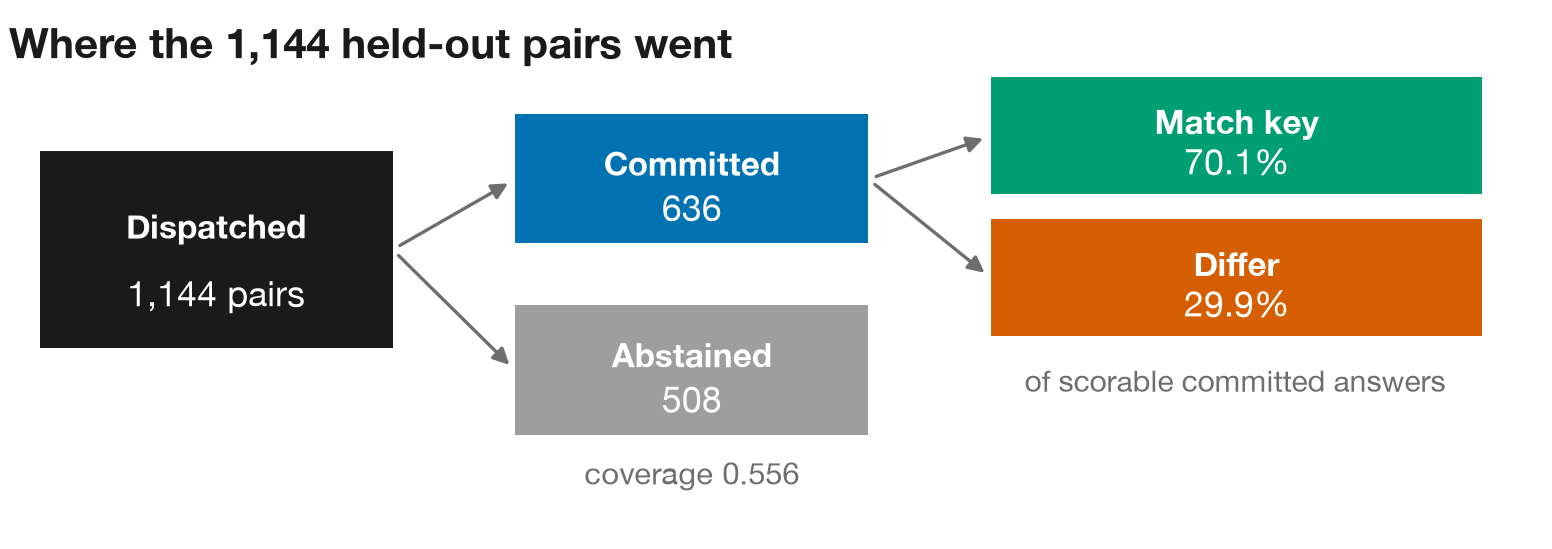
\includegraphics[width=6.1in,height=2.1578in]{media/media/image24.png}

@@CL@@Figure J.1: Where the 1,144 evaluation pairs went. 636 committed and 508 abstained, and of the scoreable commits 70.1\% match the published key.@@/CL@@

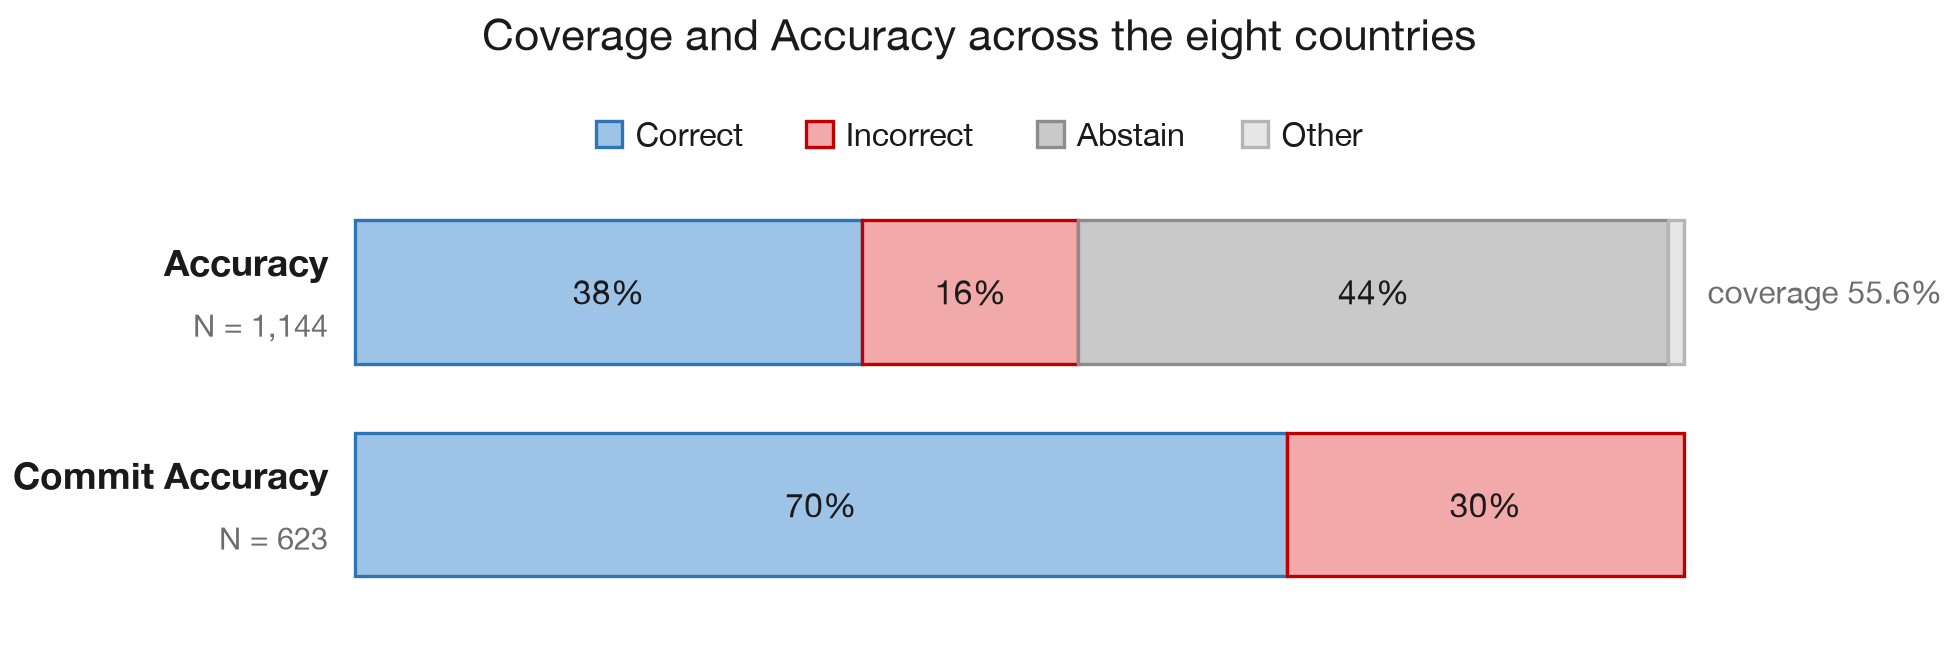
\includegraphics[width=6.1in,height=2.03126in]{media/media/image25.png}

@@CL@@Figure J.2: The evaluation run as shares of all 1,144 pairs, then of the 623 scoreable commits alone.@@/CL@@

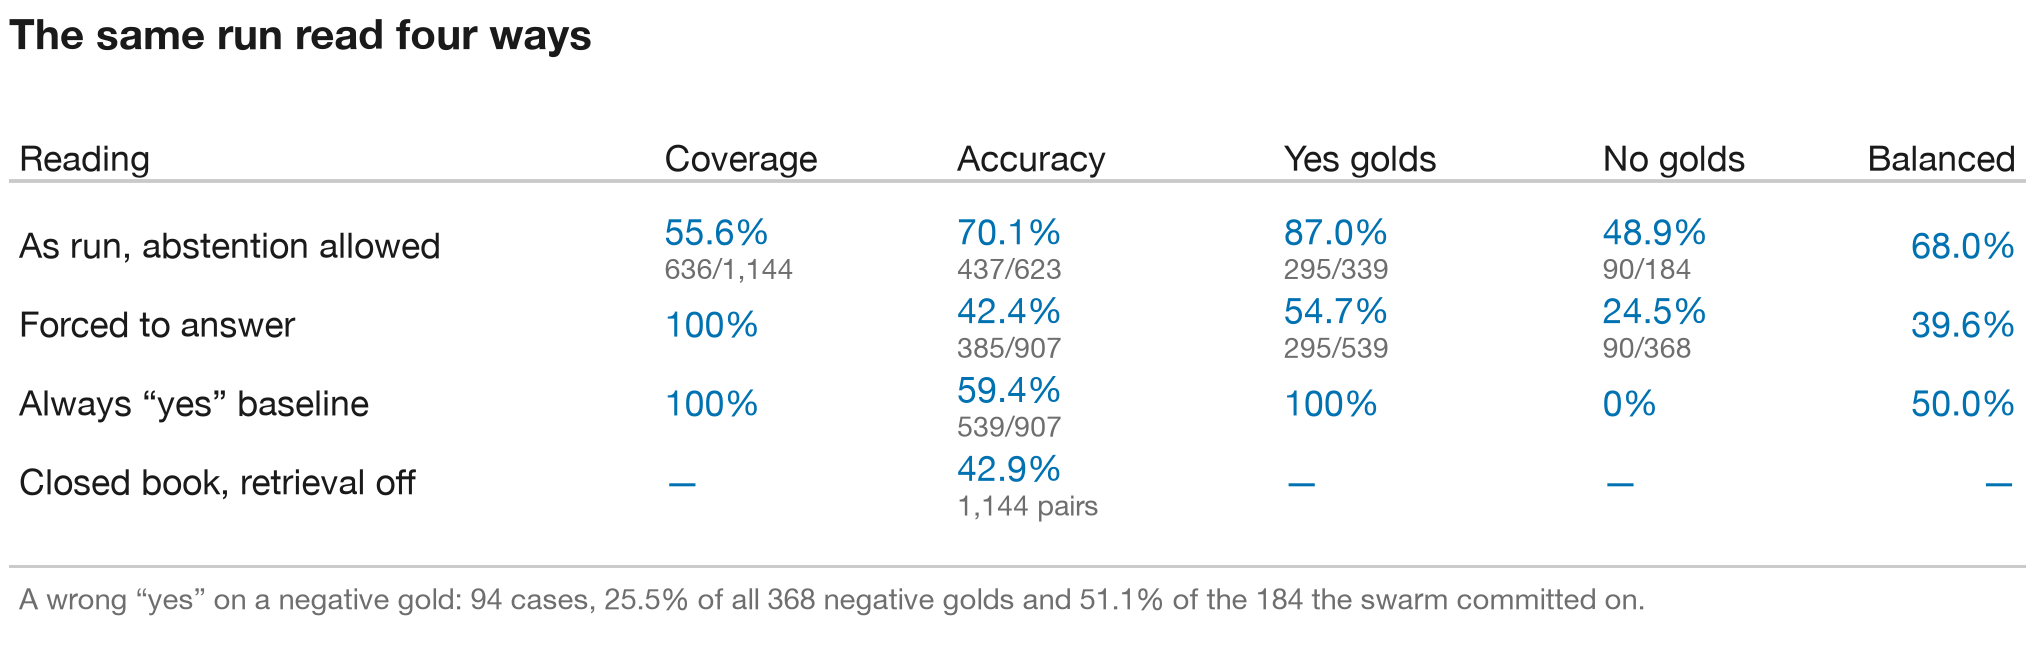
\includegraphics[width=6.1in,height=1.93641in]{media/media/image26.png}

@@CL@@Figure J.3: The same run read four ways. An alternative rendering of Table 4.1.1, with the negative-gold false-positive count underneath.@@/CL@@

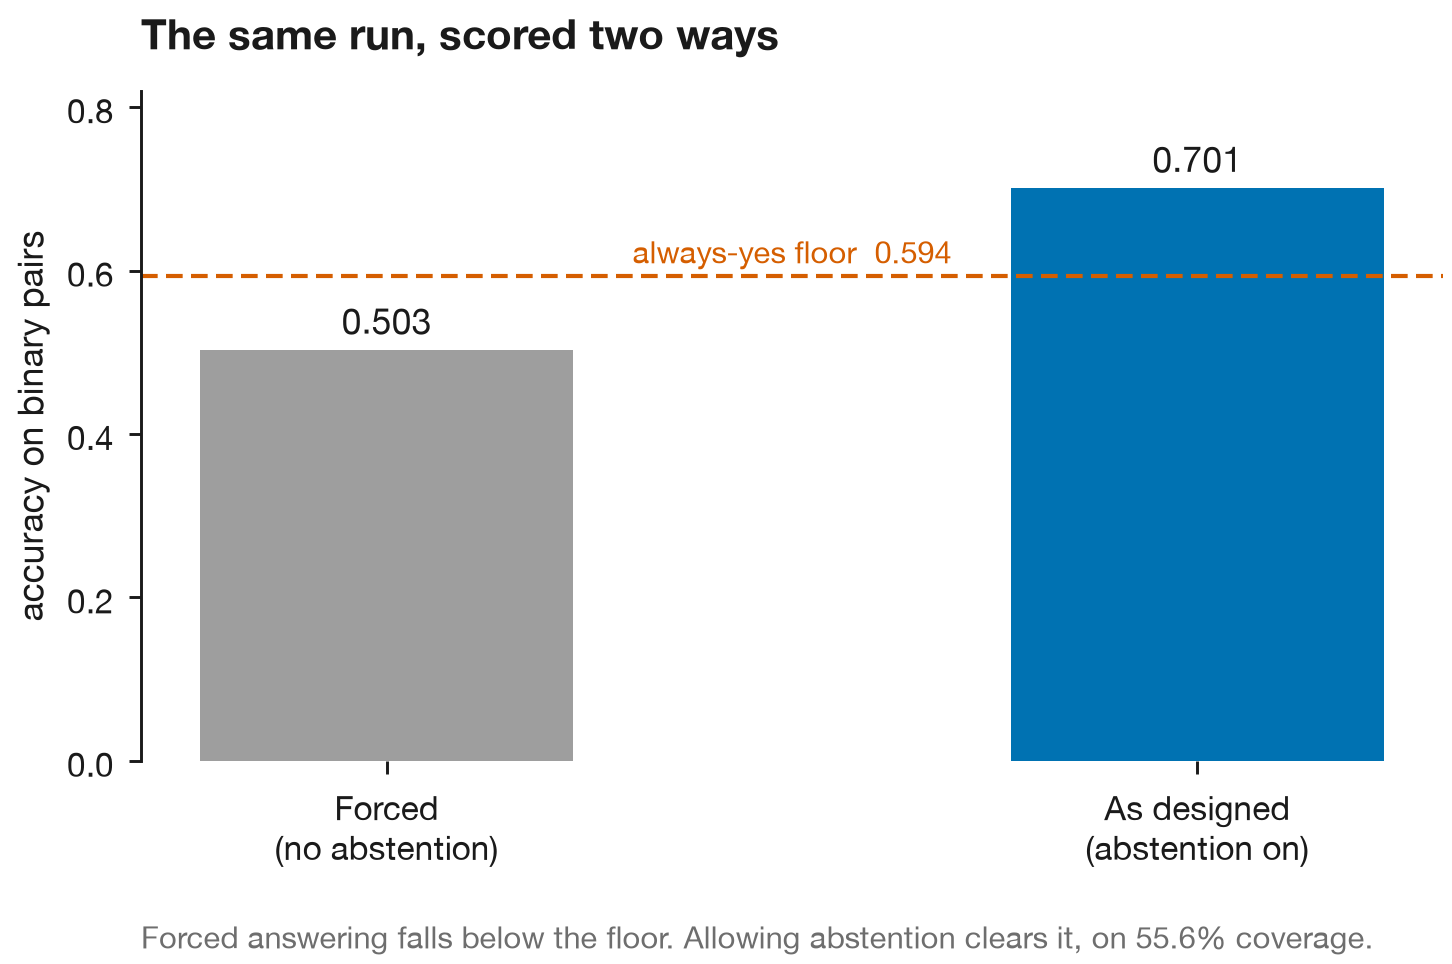
\includegraphics[width=6.09474in,height=4.04637in]{media/media/image27.png}

@@CL@@Figure J.4: Accuracy on binary pairs with abstention forced off and left on, against the always-yes floor of 0.594. Forced answering falls below the floor; allowing abstention clears it, on 55.6\% coverage.@@/CL@@

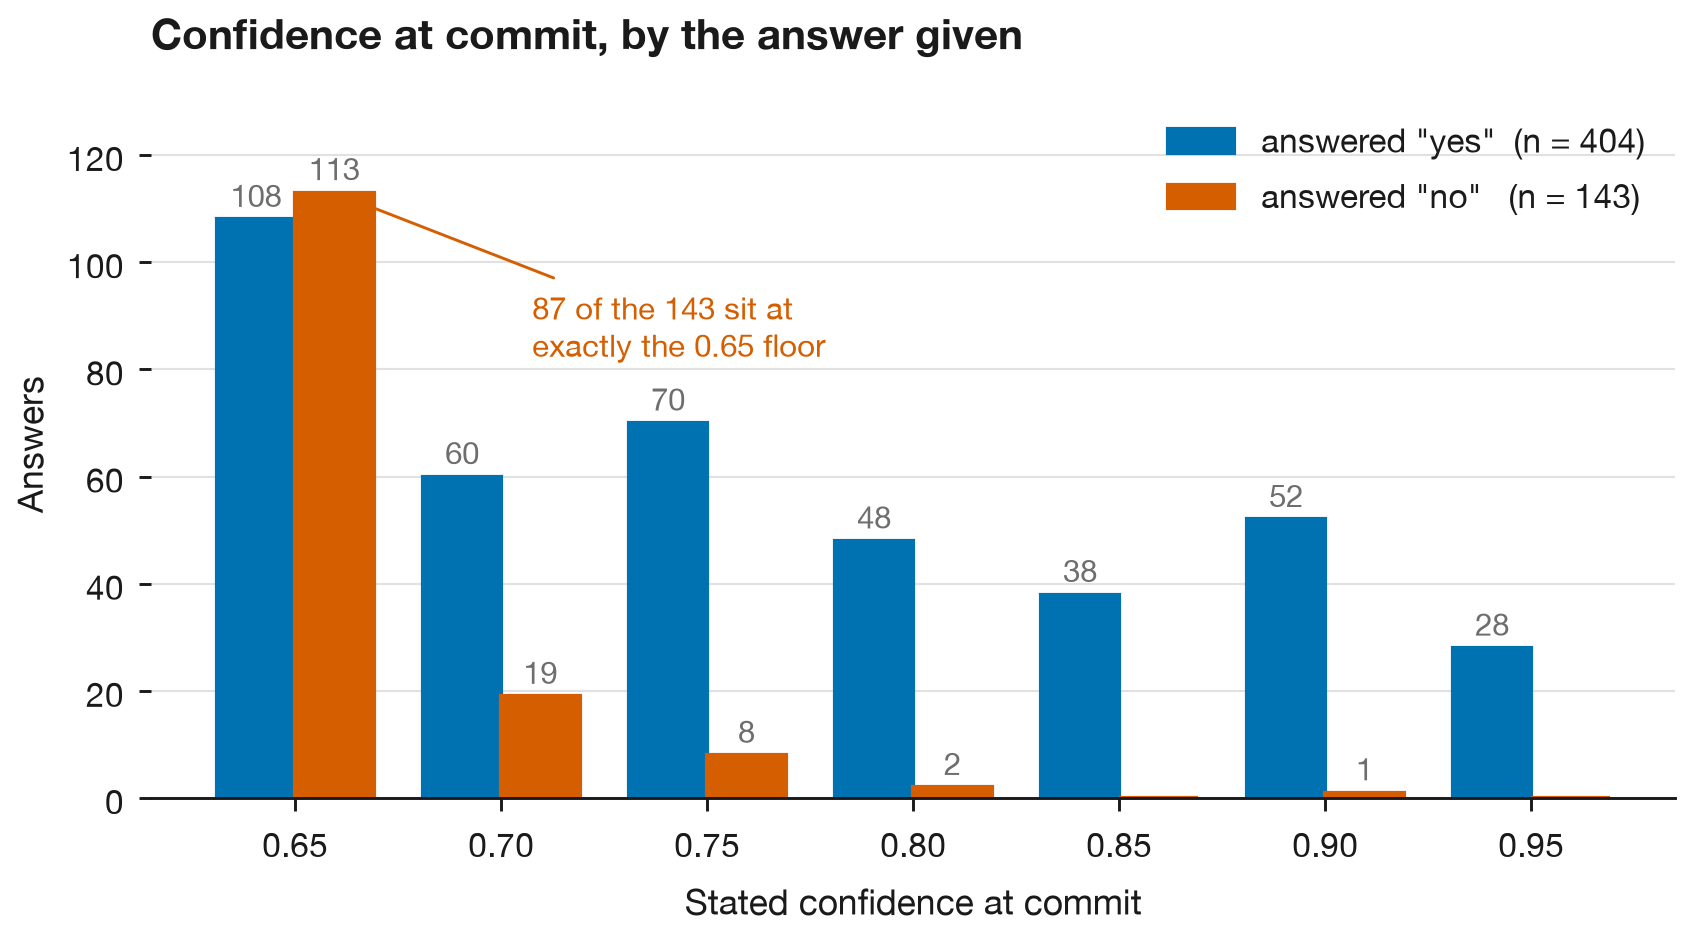
\includegraphics[width=6.1in,height=3.37239in]{media/media/image28.png}

@@CL@@Figure J.5: Stated confidence at the moment of commit, split by whether the swarm answered ``yes'' or ``no''. 87 of the 143 committed no answers sit at exactly the 0.65 floor.@@/CL@@

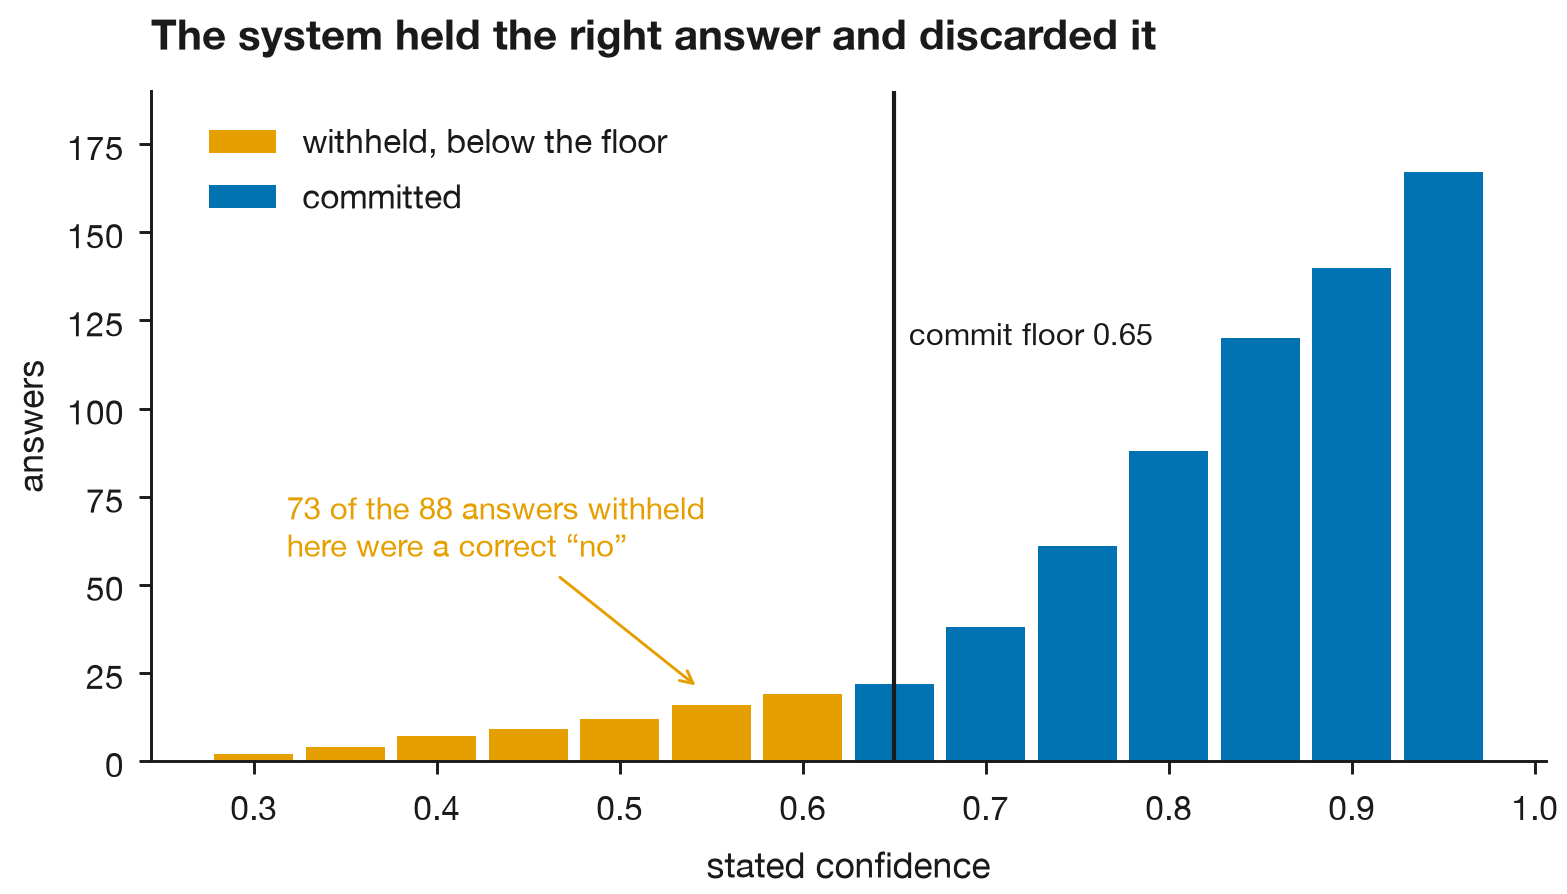
\includegraphics[width=6.1in,height=3.48015in]{media/media/image29.png}

@@CL@@Figure J.6: Answers held below the 0.65 commit floor beside those committed above it. 73 of the 88 withheld immediately under the floor were a correct no.@@/CL@@

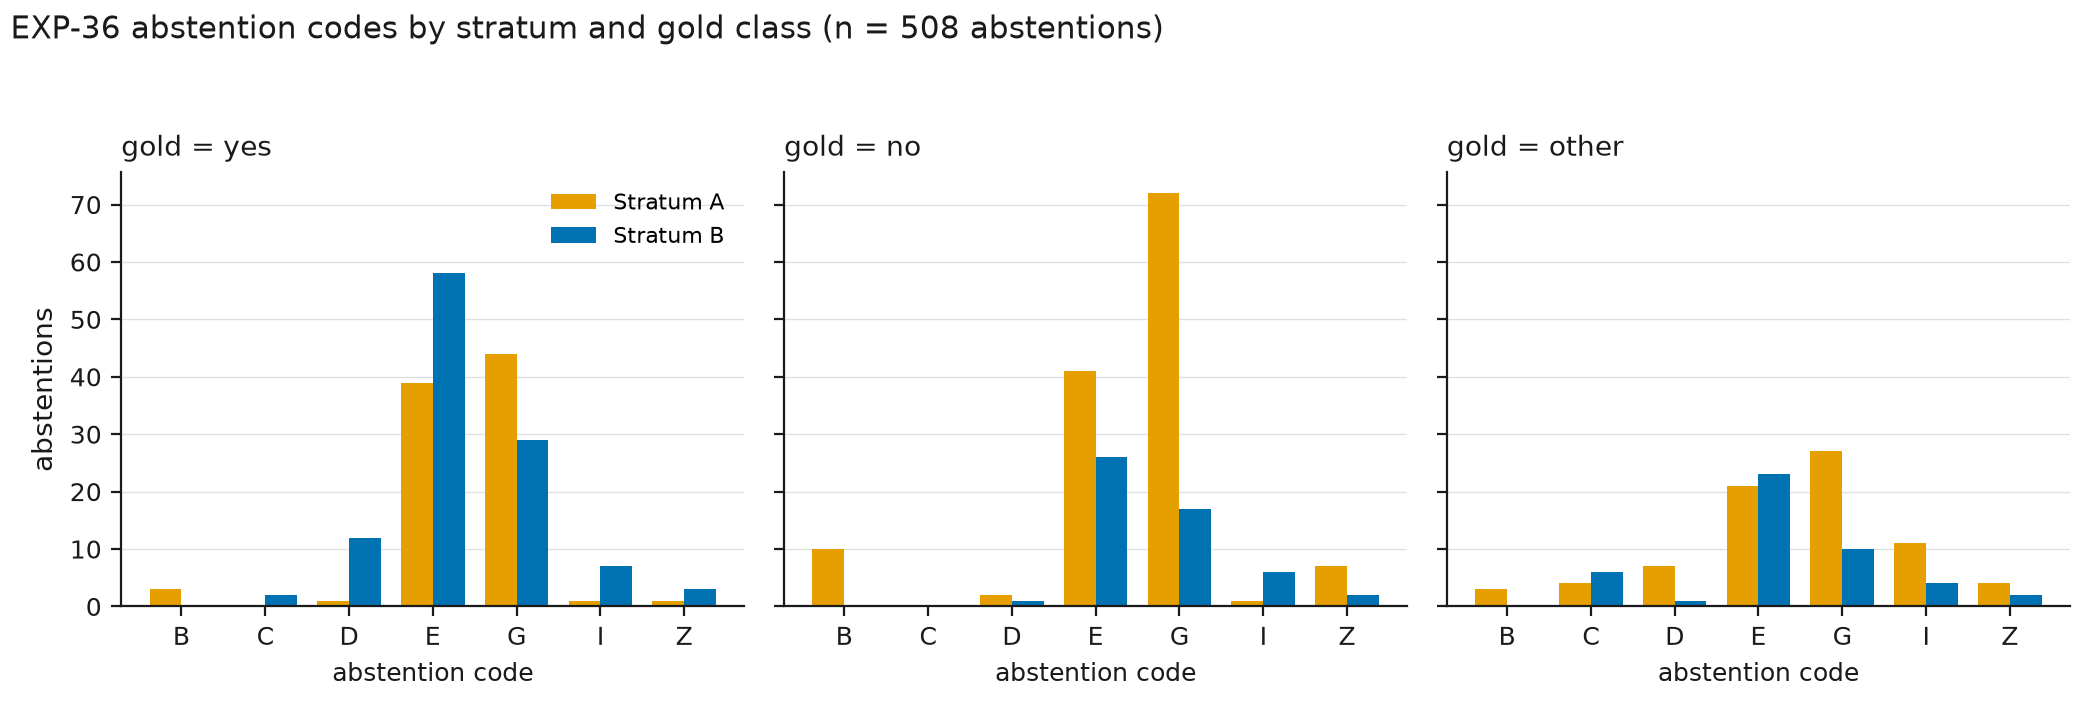
\includegraphics[width=6.1in,height=2.09143in]{media/media/image30.png}

@@CL@@Figure J.7: The 508 abstentions by code, split by resource stratum and by the class of the published answer.@@/CL@@

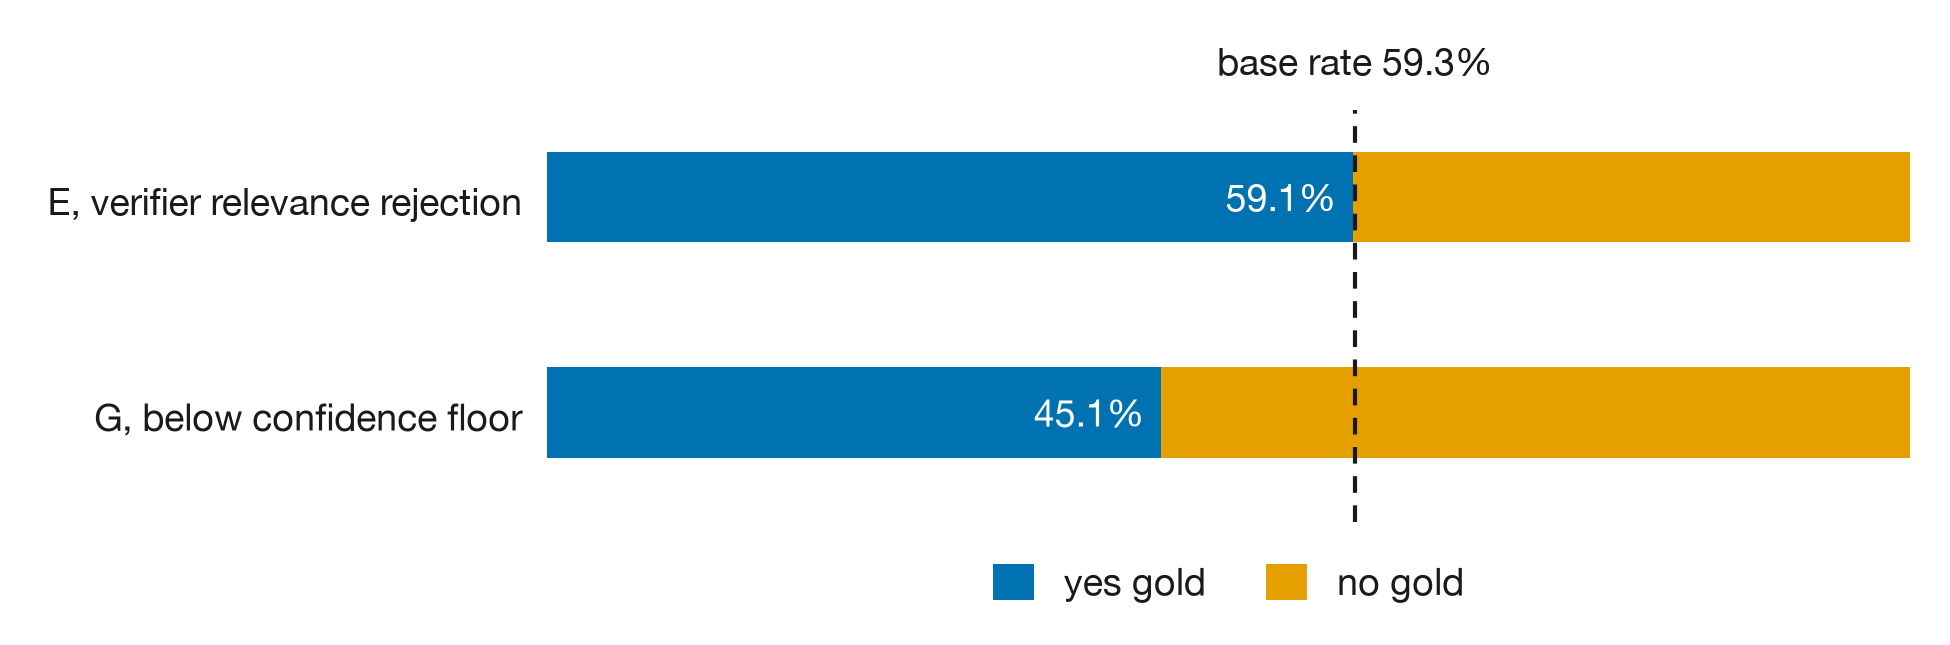
\includegraphics[width=6.1in,height=2.01769in]{media/media/image31.png}

@@CL@@Figure J.8: The gold-class mix of the two largest abstention codes against the evaluation base rate. Verifier rejections sit on the base rate at 59.1\%; floor failures are enriched in negative golds at 45.1\%.@@/CL@@

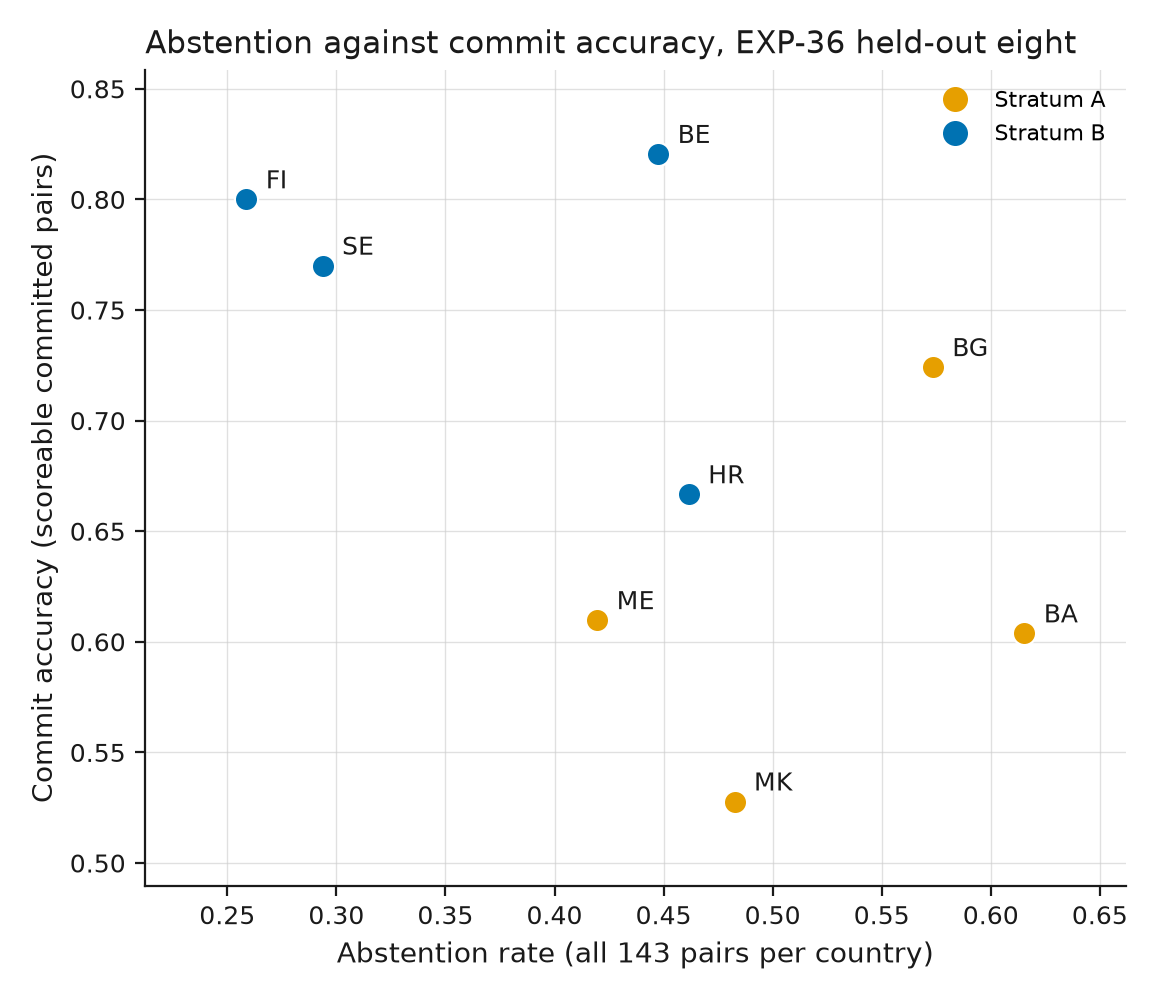
\includegraphics[width=4.69379in,height=4.04637in]{media/media/image32.png}

@@CL@@Figure J.9: Abstention rate against commit accuracy, one point per evaluation country. Abstaining more does not by itself buy accuracy.@@/CL@@

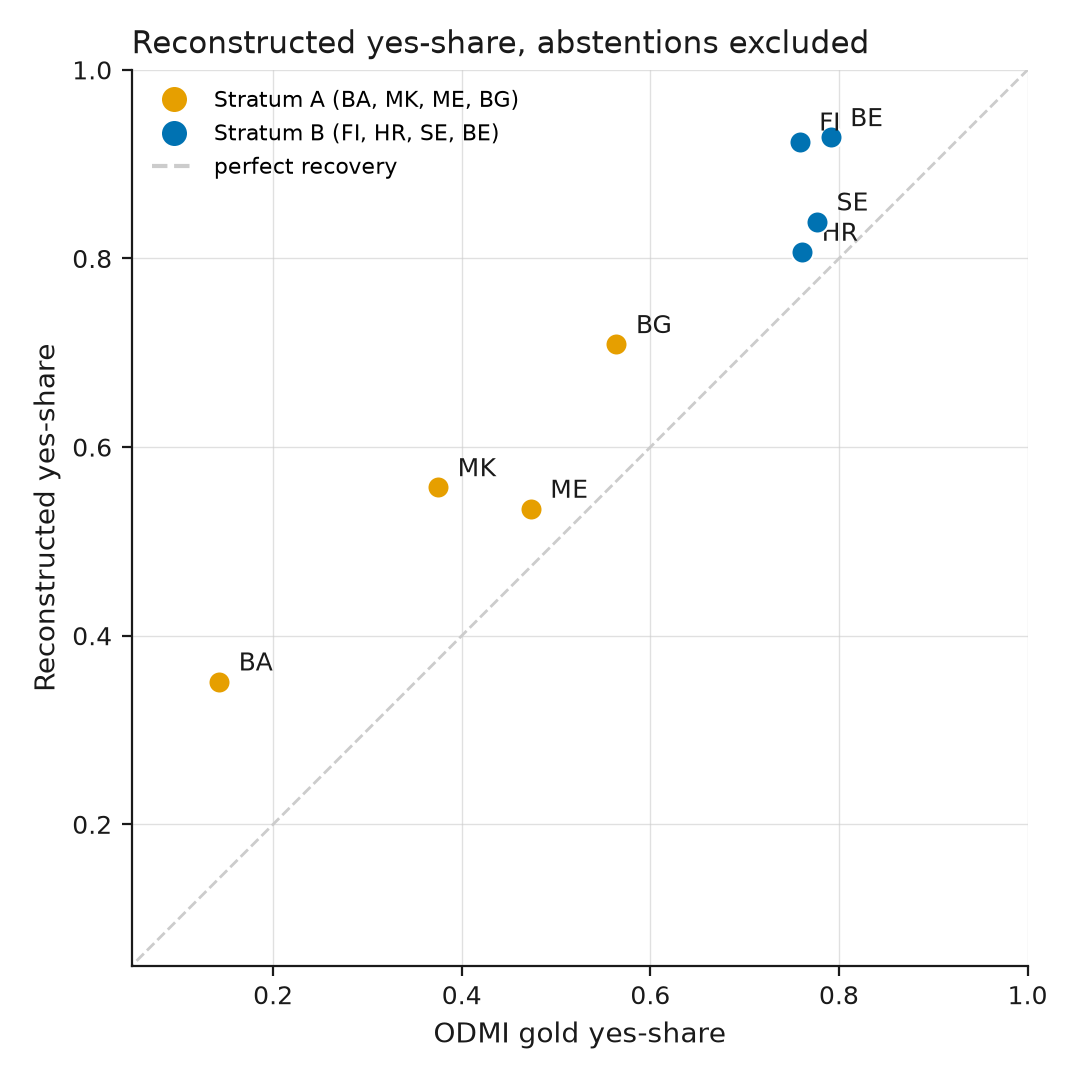
\includegraphics[width=4.04637in,height=4.04637in]{media/media/image33.png}

@@CL@@Figure J.10: Reconstructed yes-share against the published yes-share with abstentions dropped. Every country sits above the diagonal, so scoring only what the swarm answered overstates maturity.@@/CL@@

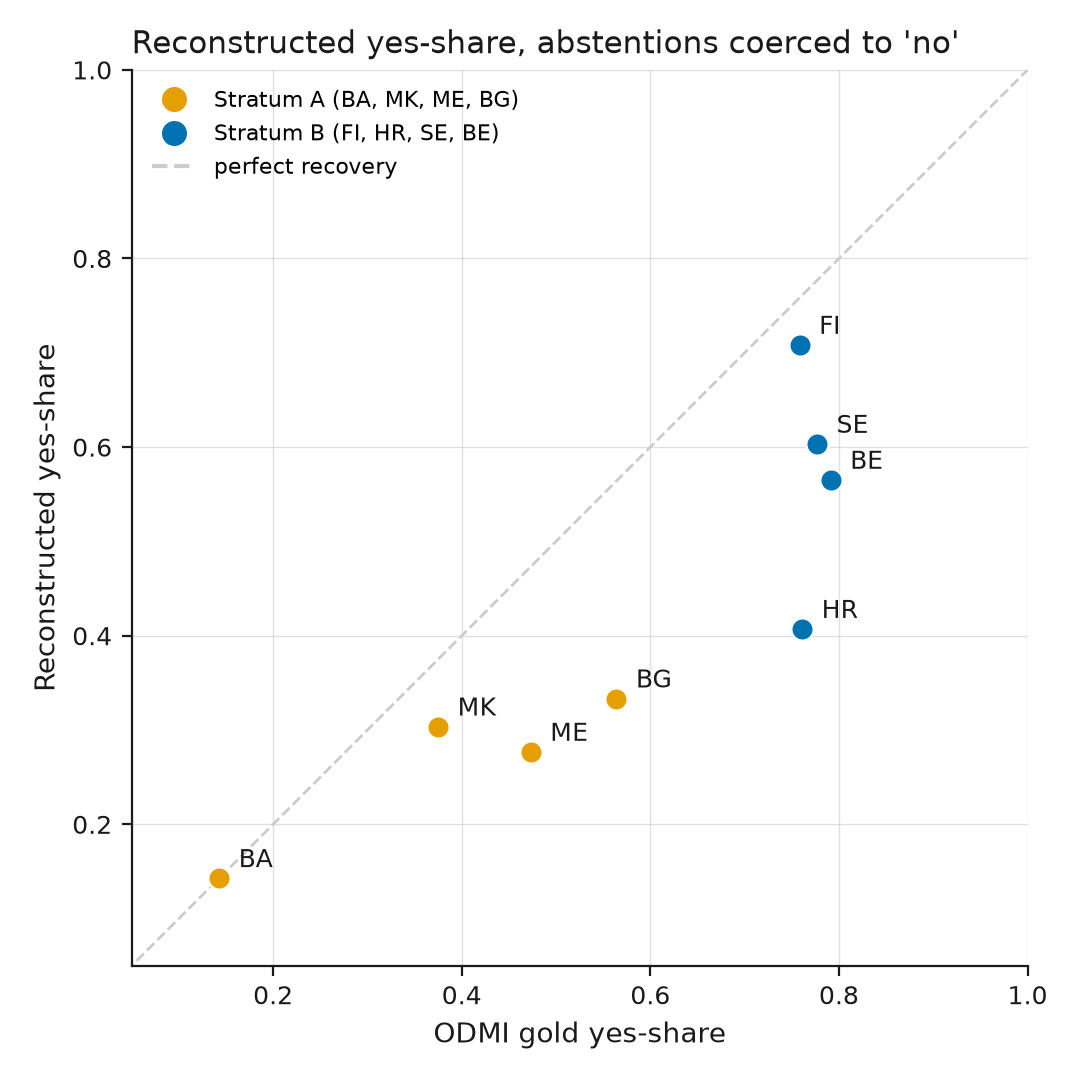
\includegraphics[width=4.04637in,height=4.04637in]{media/media/image34.png}

@@CL@@Figure J.11: The same reconstruction with every abstention coerced to no. The bias reverses and every country falls below the diagonal.@@/CL@@

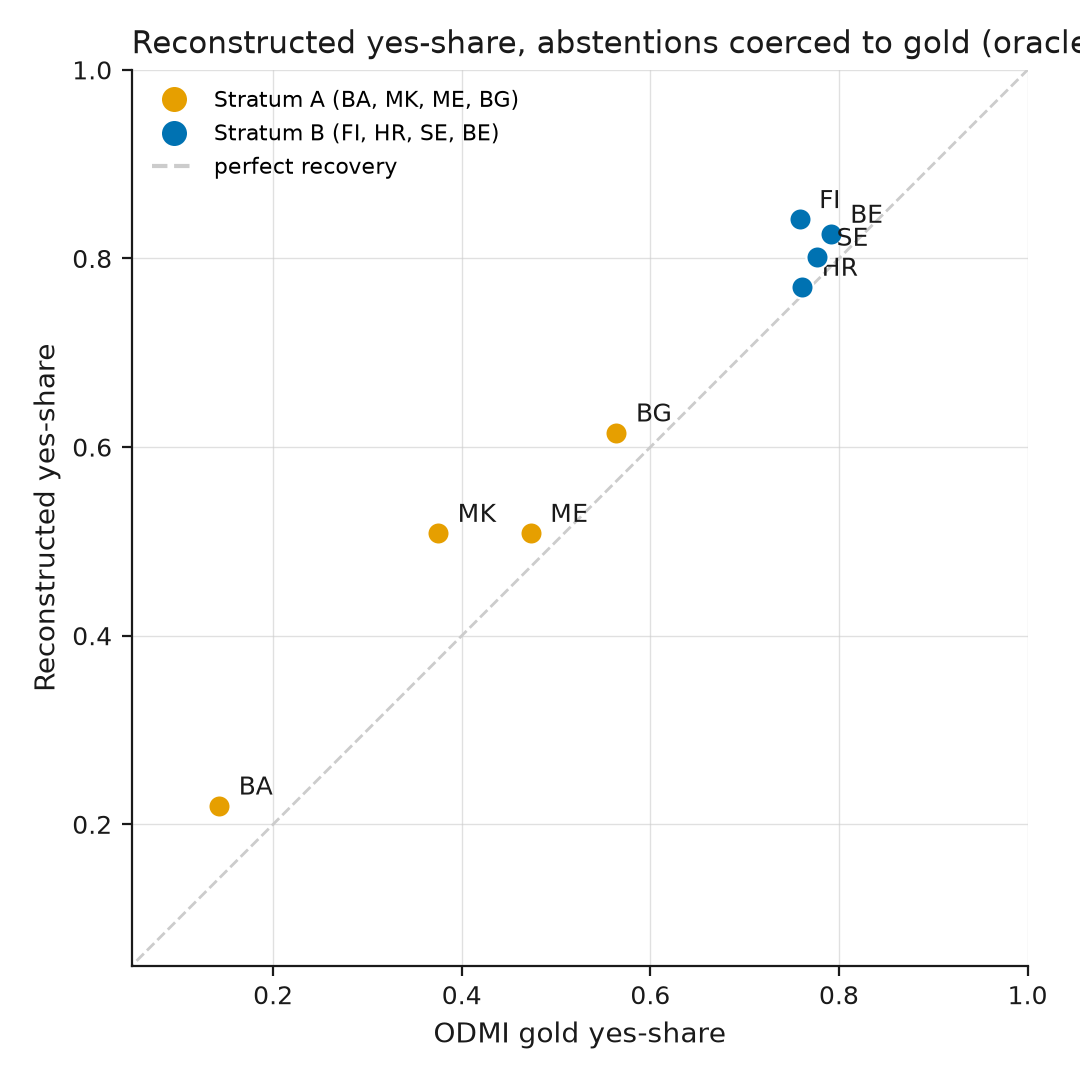
\includegraphics[width=4.04637in,height=4.04637in]{media/media/image35.png}

@@CL@@Figure J.12: The same reconstruction with abstentions filled from the published key. This is an oracle, and the ceiling the reconstruction would reach if abstention were solved.@@/CL@@

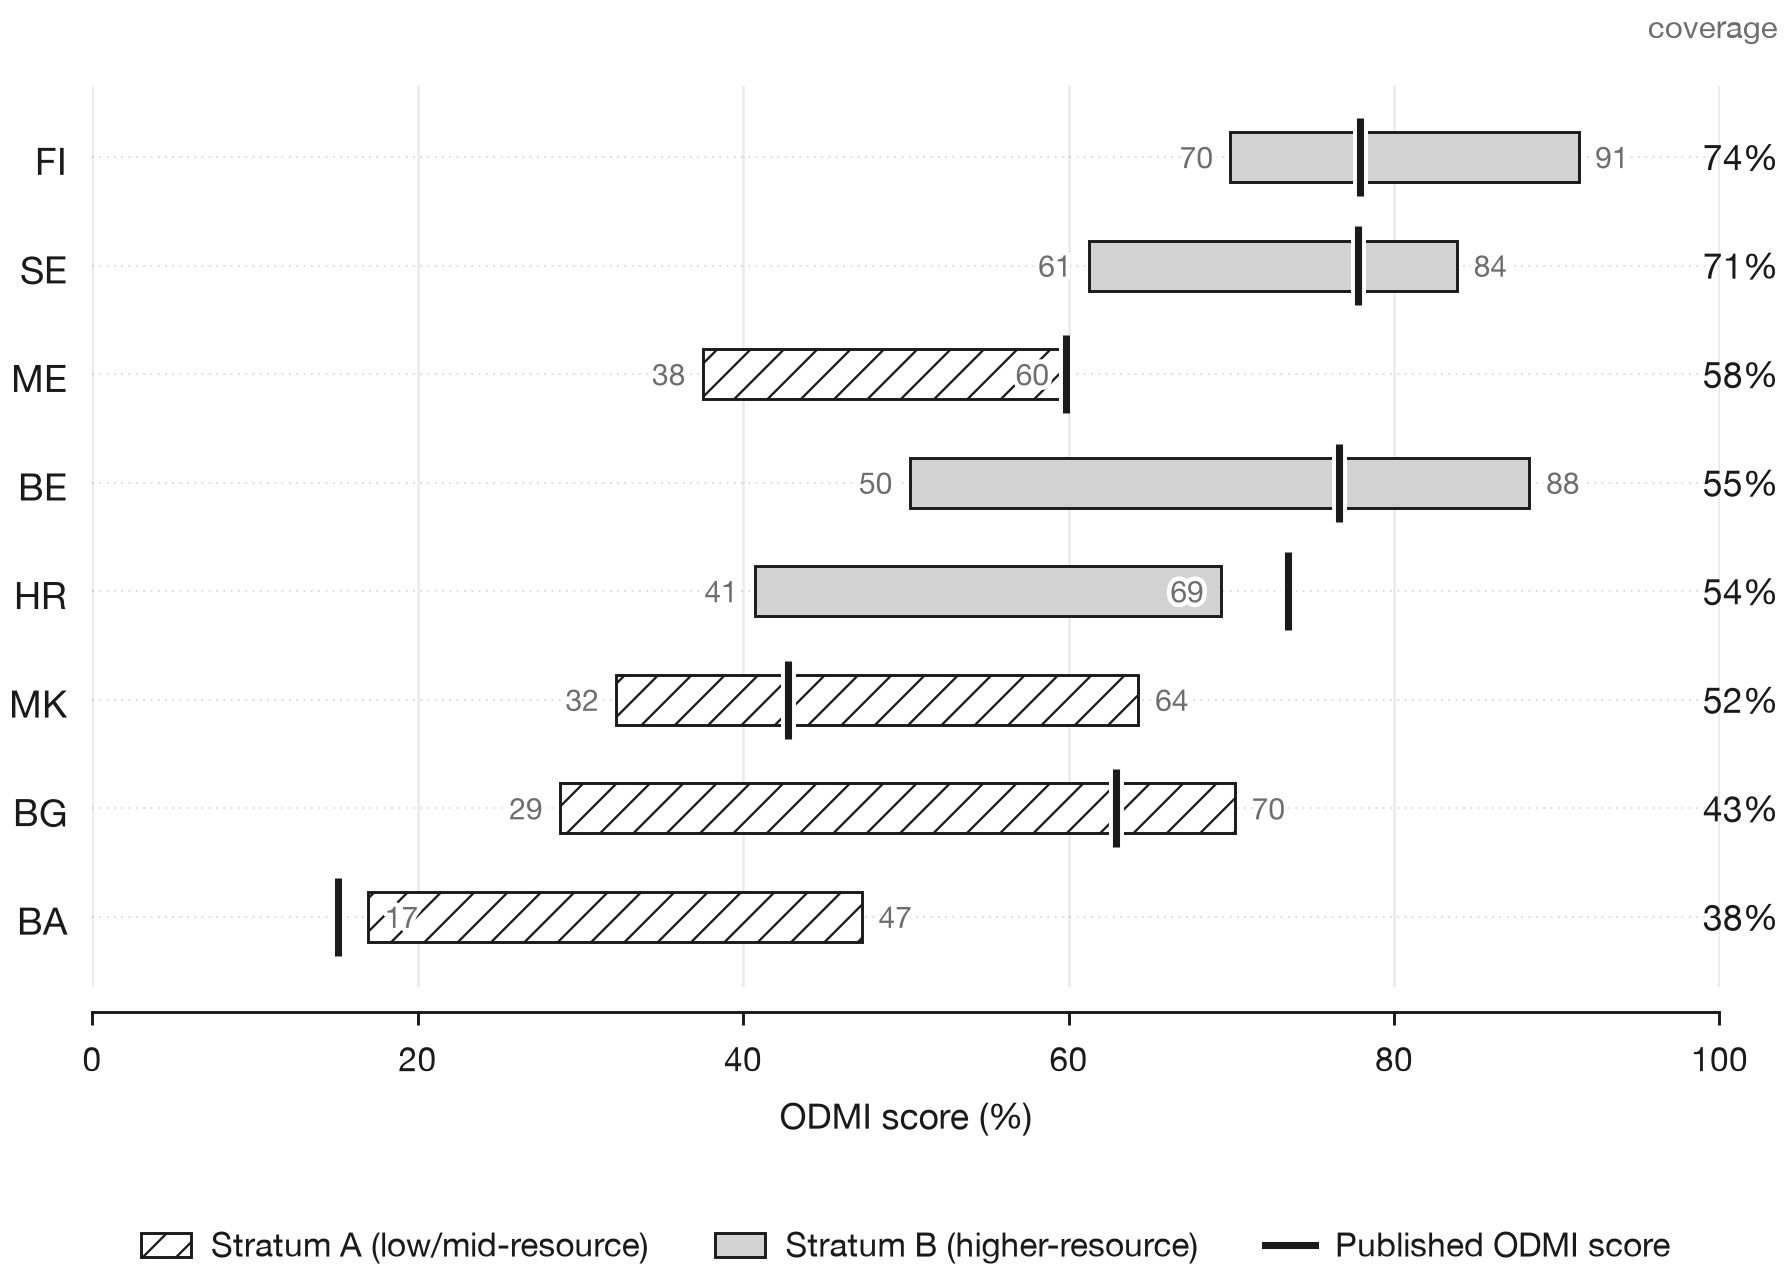
\includegraphics[width=5.61961in,height=4.04637in]{media/media/image36.png}

@@CL@@Figure J.13: The band each country\textquotesingle s reconstructed score could occupy, from treating every abstention as no to treating every one as yes, against the published score. Coverage is on the right.@@/CL@@

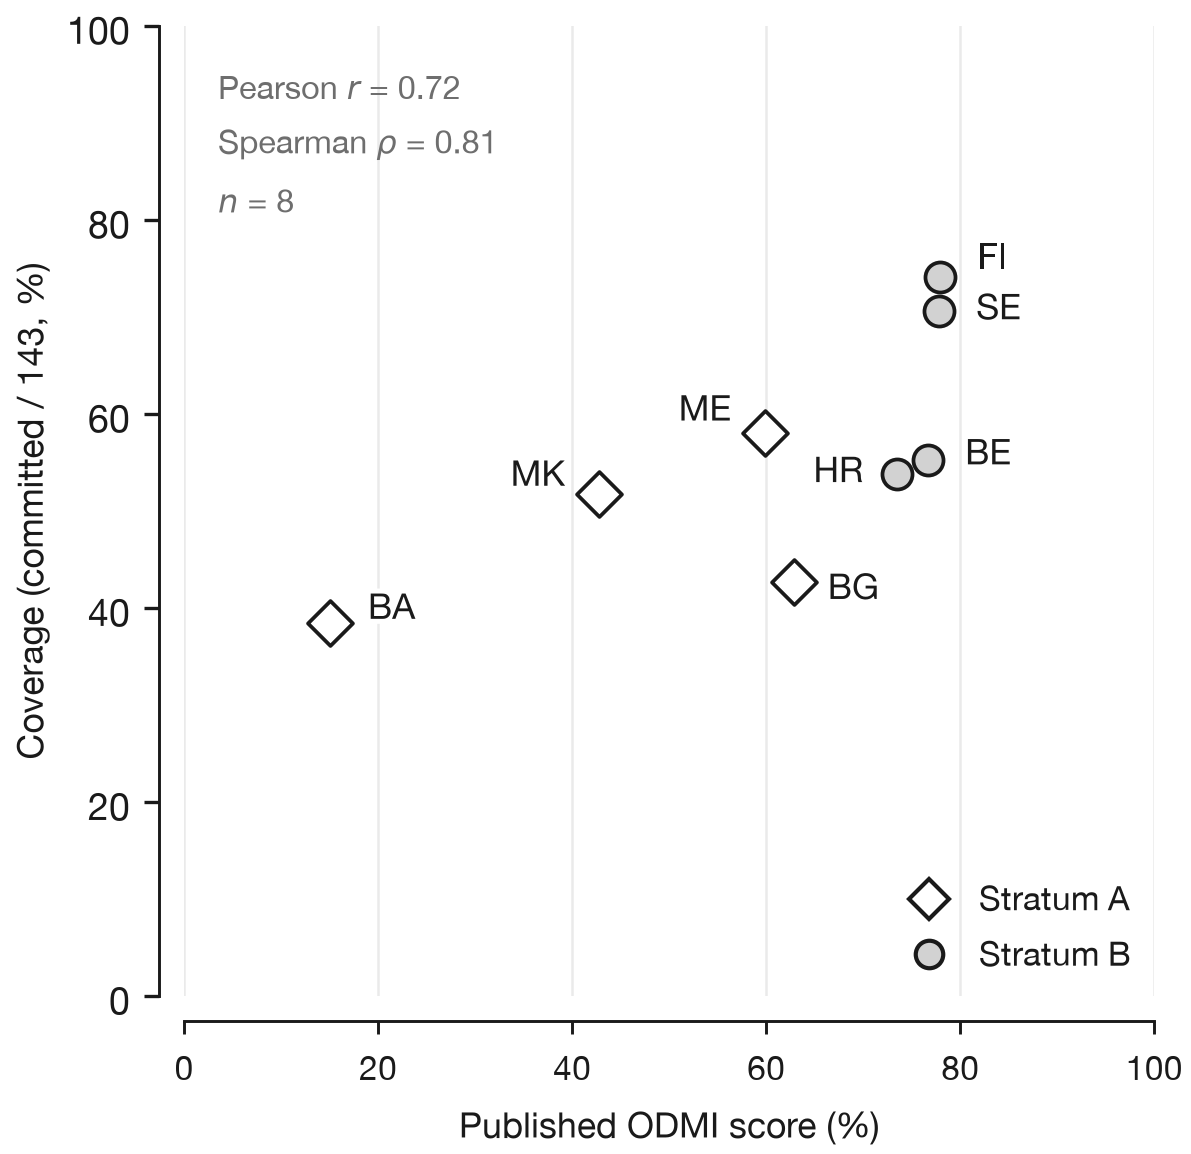
\includegraphics[width=4.17611in,height=4.04637in]{media/media/image37.png}

@@CL@@Figure J.14: Coverage against published ODMI score, one point per evaluation country, Pearson r 0.72 and Spearman rho 0.81 on eight points.@@/CL@@

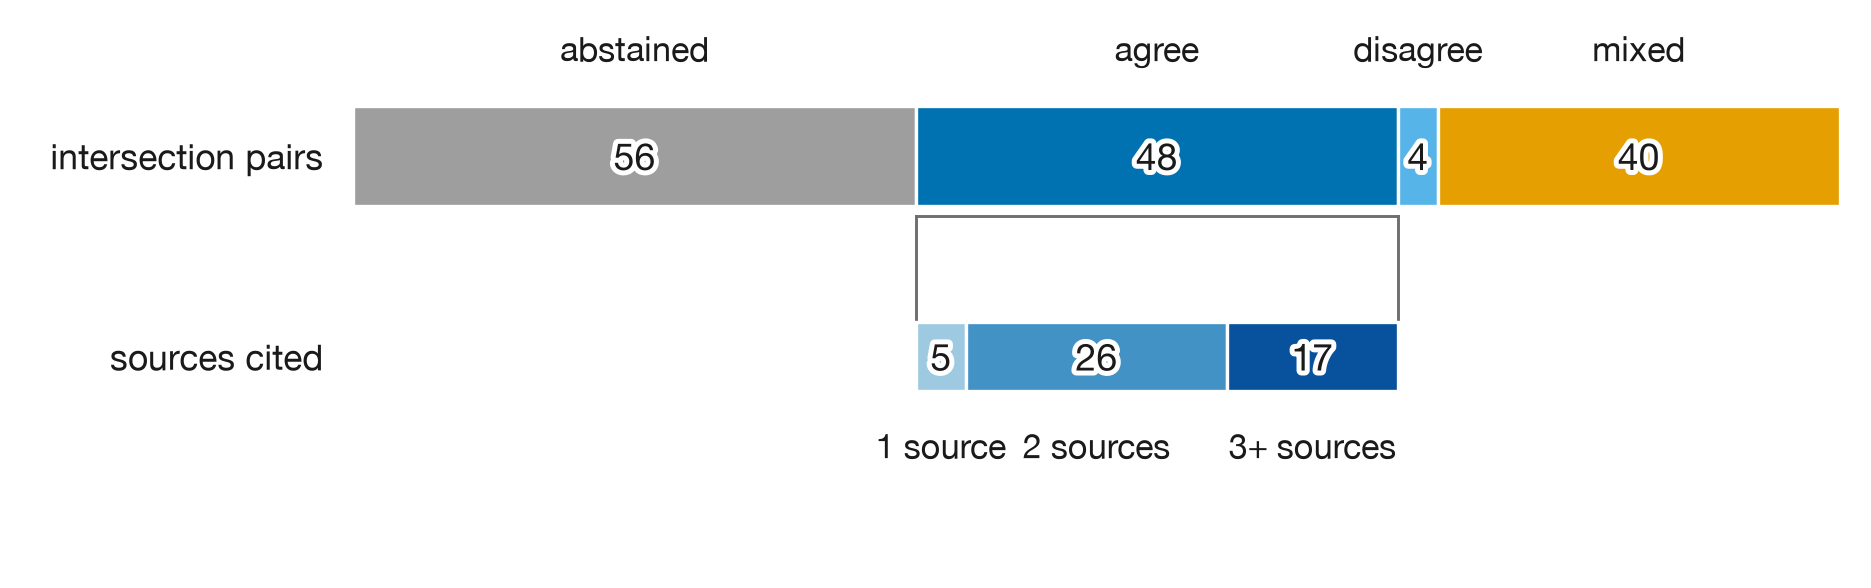
\includegraphics[width=6.1in,height=2.58382in]{media/media/image38.png}

@@CL@@Figure J.16: The two populations a human reviewer inherits. Declined answers arrive flagged and are easy to route; committed answers are identical in form whether right or wrong.@@/CL@@

@@CC@@The counts are not the evaluation run. They are the projection §4.8 makes over the full 5,148-pair questionnaire, where the evaluation coverage and commit accuracy put around 2,860 pairs committed and 2,290 declined, of which 2,010 right and 850 wrong.@@/CC@@

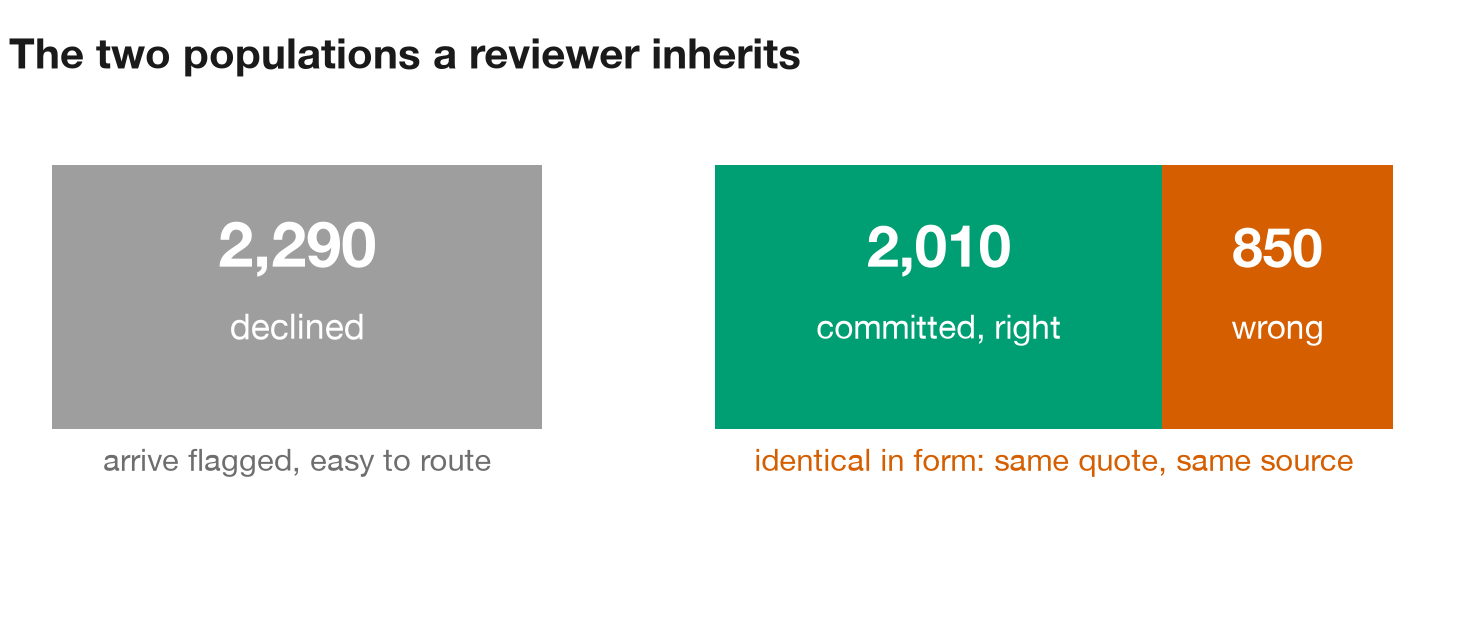
\includegraphics[width=6.1in,height=2.56865in]{media/media/image39.png}

@@CL@@Figure J.17: Why a ``yes'' and a ``no'' are not symmetric. A yes has a document behind it; a ``no'' rests on an absence, which leaves nothing to quote.@@/CL@@
